\documentclass[a4paper, 11pt, oneside]{article}

\usepackage[utf8]{inputenc}
\usepackage[T1]{fontenc}
\usepackage[french]{babel}
\usepackage{array}
\usepackage{shortvrb}
\usepackage{listings}
\usepackage[fleqn]{amsmath}
\usepackage{amsfonts}
\usepackage{fullpage}
\usepackage{enumerate}
\usepackage{graphicx}             % import, scale, and rotate graphics
\usepackage{subfigure}            % group figures
\usepackage{alltt}
\usepackage{url}
\usepackage{indentfirst}
\usepackage{eurosym}
\usepackage{listings}
\usepackage{color}
\usepackage[table,xcdraw,dvipsnames]{xcolor}

% Change le nom par défaut des listing
\renewcommand{\lstlistingname}{Extrait de Code}

\definecolor{mygray}{rgb}{0.5,0.5,0.5}
\newcommand{\coms}[1]{\textcolor{MidnightBlue}{#1}}

\lstset{
    language=C, % Utilisation du langage C
    commentstyle={\color{MidnightBlue}}, % Couleur des commentaires
    frame=single, % Entoure le code d'un joli cadre
    rulecolor=\color{black}, % Couleur de la ligne qui forme le cadre
    stringstyle=\color{RawSienna}, % Couleur des chaines de caractères
    numbers=left, % Ajoute une numérotation des lignes à gauche
    numbersep=5pt, % Distance entre les numérots de lignes et le code
    numberstyle=\tiny\color{mygray}, % Couleur des numéros de lignes
    basicstyle=\tt\footnotesize,
    tabsize=3, % Largeur des tabulations par défaut
    keywordstyle=\tt\bf\footnotesize\color{Sepia}, % Style des mots-clés
    extendedchars=true,
    captionpos=b, % sets the caption-position to bottom
    texcl=true, % Commentaires sur une ligne interprétés en Latex
    showstringspaces=false, % Ne montre pas les espace dans les chaines de caractères
    escapeinside={(>}{<)}, % Permet de mettre du latex entre des <( et )>.
    inputencoding=utf8,
    literate=
  {á}{{\'a}}1 {é}{{\'e}}1 {í}{{\'i}}1 {ó}{{\'o}}1 {ú}{{\'u}}1
  {Á}{{\'A}}1 {É}{{\'E}}1 {Í}{{\'I}}1 {Ó}{{\'O}}1 {Ú}{{\'U}}1
  {à}{{\`a}}1 {è}{{\`e}}1 {ì}{{\`i}}1 {ò}{{\`o}}1 {ù}{{\`u}}1
  {À}{{\`A}}1 {È}{{\`E}}1 {Ì}{{\`I}}1 {Ò}{{\`O}}1 {Ù}{{\`U}}1
  {ä}{{\"a}}1 {ë}{{\"e}}1 {ï}{{\"i}}1 {ö}{{\"o}}1 {ü}{{\"u}}1
  {Ä}{{\"A}}1 {Ë}{{\"E}}1 {Ï}{{\"I}}1 {Ö}{{\"O}}1 {Ü}{{\"U}}1
  {â}{{\^a}}1 {ê}{{\^e}}1 {î}{{\^i}}1 {ô}{{\^o}}1 {û}{{\^u}}1
  {Â}{{\^A}}1 {Ê}{{\^E}}1 {Î}{{\^I}}1 {Ô}{{\^O}}1 {Û}{{\^U}}1
  {œ}{{\oe}}1 {Œ}{{\OE}}1 {æ}{{\ae}}1 {Æ}{{\AE}}1 {ß}{{\ss}}1
  {ű}{{\H{u}}}1 {Ű}{{\H{U}}}1 {ő}{{\H{o}}}1 {Ő}{{\H{O}}}1
  {ç}{{\c c}}1 {Ç}{{\c C}}1 {ø}{{\o}}1 {å}{{\r a}}1 {Å}{{\r A}}1
  {€}{{\euro}}1 {£}{{\pounds}}1 {«}{{\guillemotleft}}1
  {»}{{\guillemotright}}1 {ñ}{{\~n}}1 {Ñ}{{\~N}}1 {¿}{{?`}}1
}

%%%%%%%%%%%%%%%%% TITRE %%%%%%%%%%%%%%%%
% Complétez et décommentez les définitions de macros suivantes :
 \newcommand{\intitule}{Five or more}
 \newcommand{\GrNbr}{07}
 \newcommand{\PrenomUN}{Lucas}
 \newcommand{\NomUN}{Lolo}
 \newcommand{\PrenomDEUX}{Marzouk}
 \newcommand{\NomDEUX}{Ouro-Gomma}


%%%%%%%% ZONE PROTÉGÉE : MODIFIEZ UNE DES DIX PROCHAINES %%%%%%%%
%%%%%%%%            LIGNES POUR PERDRE 2 PTS.            %%%%%%%%

\title{INFO0030: \intitule}
\author{Groupe \GrNbr : \PrenomUN~\textsc{\NomUN}, \PrenomDEUX~\textsc{\NomDEUX}}
\date{}

\begin{document}

\maketitle
\newpage
\tableofcontents
\newpage
%%%%%%%%%%%%%%%%%%%% FIN DE LA ZONE PROTÉGÉE %%%%%%%%%%%%%%%%%%%%

%%%%%%%%%%%%%%%% RAPPORT %%%%%%%%%%%%%%%
% Écrivez votre rapport ci-dessous.
\section{Architecture générale du code}
Pour l'architecture générale du code nous avons utilisé le pattern MVC.\\ \\
\subsection{Le Modèle}
Contient les fonctionnalités de l'application, qui agissent sur la structure pour modifier ses informations et son contenu.
\\ \\
\subsection{La Vue}
Contient les fonctions qui modifient les éléments à afficher sur la fenêtre de l'application.
\\ \\
\subsection{Le Controleur}
Contient les fonctions qui font le lien entre les entrées externes "click" et le modèle qui contient les données.
\\ \\
\subsection{Interaction}
Notre code utilise trois structures de données, une pour les données de jeu, une autre pour les éléments visuels (images) et la dernière combine les deux structures mentionnées précédemment.
La partie modèle rassemble les données d'exploitation sans modifier l'effet visuel, tandis que la partie vue modifie les éléments en raison des données.Enfin, le contrôleur transforme l'opération de l'utilisateur en une opération sur le modèle.
\newpage
\section{Les structures de données}
\subsection{Structure ModeleFive}
%%%%%%%%%%%%%%%%%%%%%%%%%%%%%%%%%%%%%%%%%%%%%%%%%%%%%%
\begin{lstlisting}[caption={Structure modele}]
typedef struct modele_t{
    int niveau; //Contient le niveau choisit.
    int largeur; //Contient la largeur de la grille.
    int hauteur; //Contient la hauteur de la grille.
    int typeSymboles; //Contient le nombre de couleur au cours de la partie.
    int symbolesTour; //Contient le nombre de symbole a ajouté à chaque tour.
    int cellules; //Contient le nombre de case de la grille.
    int grille[20][15]; //Une grille contenant la couleur d'une image.
    int aleatoire[20][15]; //Une grille contenant les positions des cases blanches.
    int combo; //Contient le combo maximale.
    int avancer_tableau_horizontale; //Permet d'avancer pour la victoire d'un combo.
    int avancer_tableau_verticale; //Permet d'avancer pour la victoire d'un combo.
    int avancer_tableau_oblique; //Permet d'avancer pour la victoire d'un combo.
    int oblique_decroissant; //Permet d'avancer pour la victoire d'un combo.
    int score; //Contient le score courant de l'utilisateur.
    int ligneActuelle[10]; //Contient les 10 meilleures scores de l'utilisateur.
    int nouvelle_partie; //Permet de savoir combien de partie ont été jouée.
}ModeleFive;
\end{lstlisting}
\textbf{La structure ModeleFive:}\\ 
Nous permet de stocker les informations propre du modele.
\\ \\
\textbf{Pertinence:}\\
Cette structure nous permet de l'utiliser pour obtenir des informations au cours du jeu. Les champs sont détailles ci-dessus. Le cout des informations en "int" est sensée car nous stockons uniquement des nombres.

\subsection{Structure VueFive}
%%%%%%%%%%%%%%%%%%%%%%%%%%%%%%%%%%%%%%%%%%%%%%%%
\begin{lstlisting}[caption={Structure vue}]
typedef struct vue_t{
    ModeleFive *mf; 
    GtkWidget **image; //Contient le nombre d'image a chargé et a modifié.
    GtkWidget **image_aleatoire; //Contient le nombre d'image a chargé et a modifié pour les informations prochaines.
    GtkWidget **bouton_aleatoire; //Contient le nombre de bouton pour les informations prochaines.
    GtkWidget *Score; //Permet d'afficher le score sur le tableau de bord.
    int couleur_actuelle[7]; //Est la position du bouton qui donne les informations.
}VueFive;
\end{lstlisting}
\textbf{La structure VueFive:}\\ 
Contient les éléments visuels du jeu qui sont aussi expliqués ci-dessus.
\\ \\
\textbf{Pertinence:}\\
 Utilisation des malloc pour les widgets semblent une bonne idée. 

\newpage
\subsection{Structure ControleurFive}
%%%%%%%%%%%%%%%%%%%%%%%%%%%%%%%%%%%%%%%%%%%%%%%%%%%%%
\begin{lstlisting}[caption={Structure controleur}]
typedef struct controleur_t{
    VueFive *vf; 
    ModeleFive *mf; 
    GtkWidget **bouton; //Contient le nombre de bouton dans le jeu.
    GtkWidget *Fenetre; //Est la fenêtre courante du jeu.
    char *fichier_score; //Est le fichier de l'utilisateur.
    int nombre; //Permet de savoir si l'utilisateur a bien fait les deux clicks.
    int x_init; //Contient la coordonnée horizontale du premier click.
    int y_init; //Contient la coordonnée verticale du premier click.
    int x_dest; //Contient la coordonnée horizontale du deuxieme click.
    int y_dest; //Contient la coordonnée verticale du deuxieme click.
}ControleurFive;
\end{lstlisting}
\textbf{La structure ControleurFive:}\\
contient l'ensemble des autres structures puisqu'elle doit les mettre en lien avec les intéraction de l'utilisateur.\\ \\
\textbf{Pertinence:}\\
une structure qui rassemble toutes les autres est très utile dans un jeu aussi complexe que le jeu five or more. Petit bémol, le fichier n'a pas été utilisé par soucis de temps ou le mal compris de l'énoncé.
\newpage

\section{Les algorithmes particuliers}
%%%%%%%%%%%%%%%%%%%%%%%%%%%%%%%%%%%%%%%%%%%%%%%%%%%%%
\subsection{Déplacement (labyrinthe)}
\begin{lstlisting}
int deplacement(ControleurFive *cf){
  voir ControleurFive.c 
}

\end{lstlisting}
\textbf{Idée:}\\
Cette algorithme a pour but de déplacer une image d'un endroit à l'autre du plateau si le chemin existe.
\\
\textbf{Implémentation:}\\
Cette algorithme est composé de 4 parties importantes qui servent à déplacer l'image en foncion de sa destination(monter à gauche ou droite ou descendre à gauche ou droite). L'algorithme se dirigera toujours vers la destination la plus proche et donc prendra seulement un chemin différent si le chemin le plus court s'avère bloquer.


\subsection{Vérification horizontale}
\begin{lstlisting}
int verification_horizontale( ControleurFive *cf){
    for(int ComboAll = cf->mf->combo ; ComboAll >= 5 ; ComboAll--){
        for(int k = 0; k < cf->mf->avancer_tableau_horizontale; k++){
            for(int i = 0; i < cf->mf->hauteur; i++){
                for(int j = 1; j < cf->mf->typeSymboles+1; j++){
                }
                //Avec tous les if
            }
        }
    }
}
\end{lstlisting}
\begin{center}
    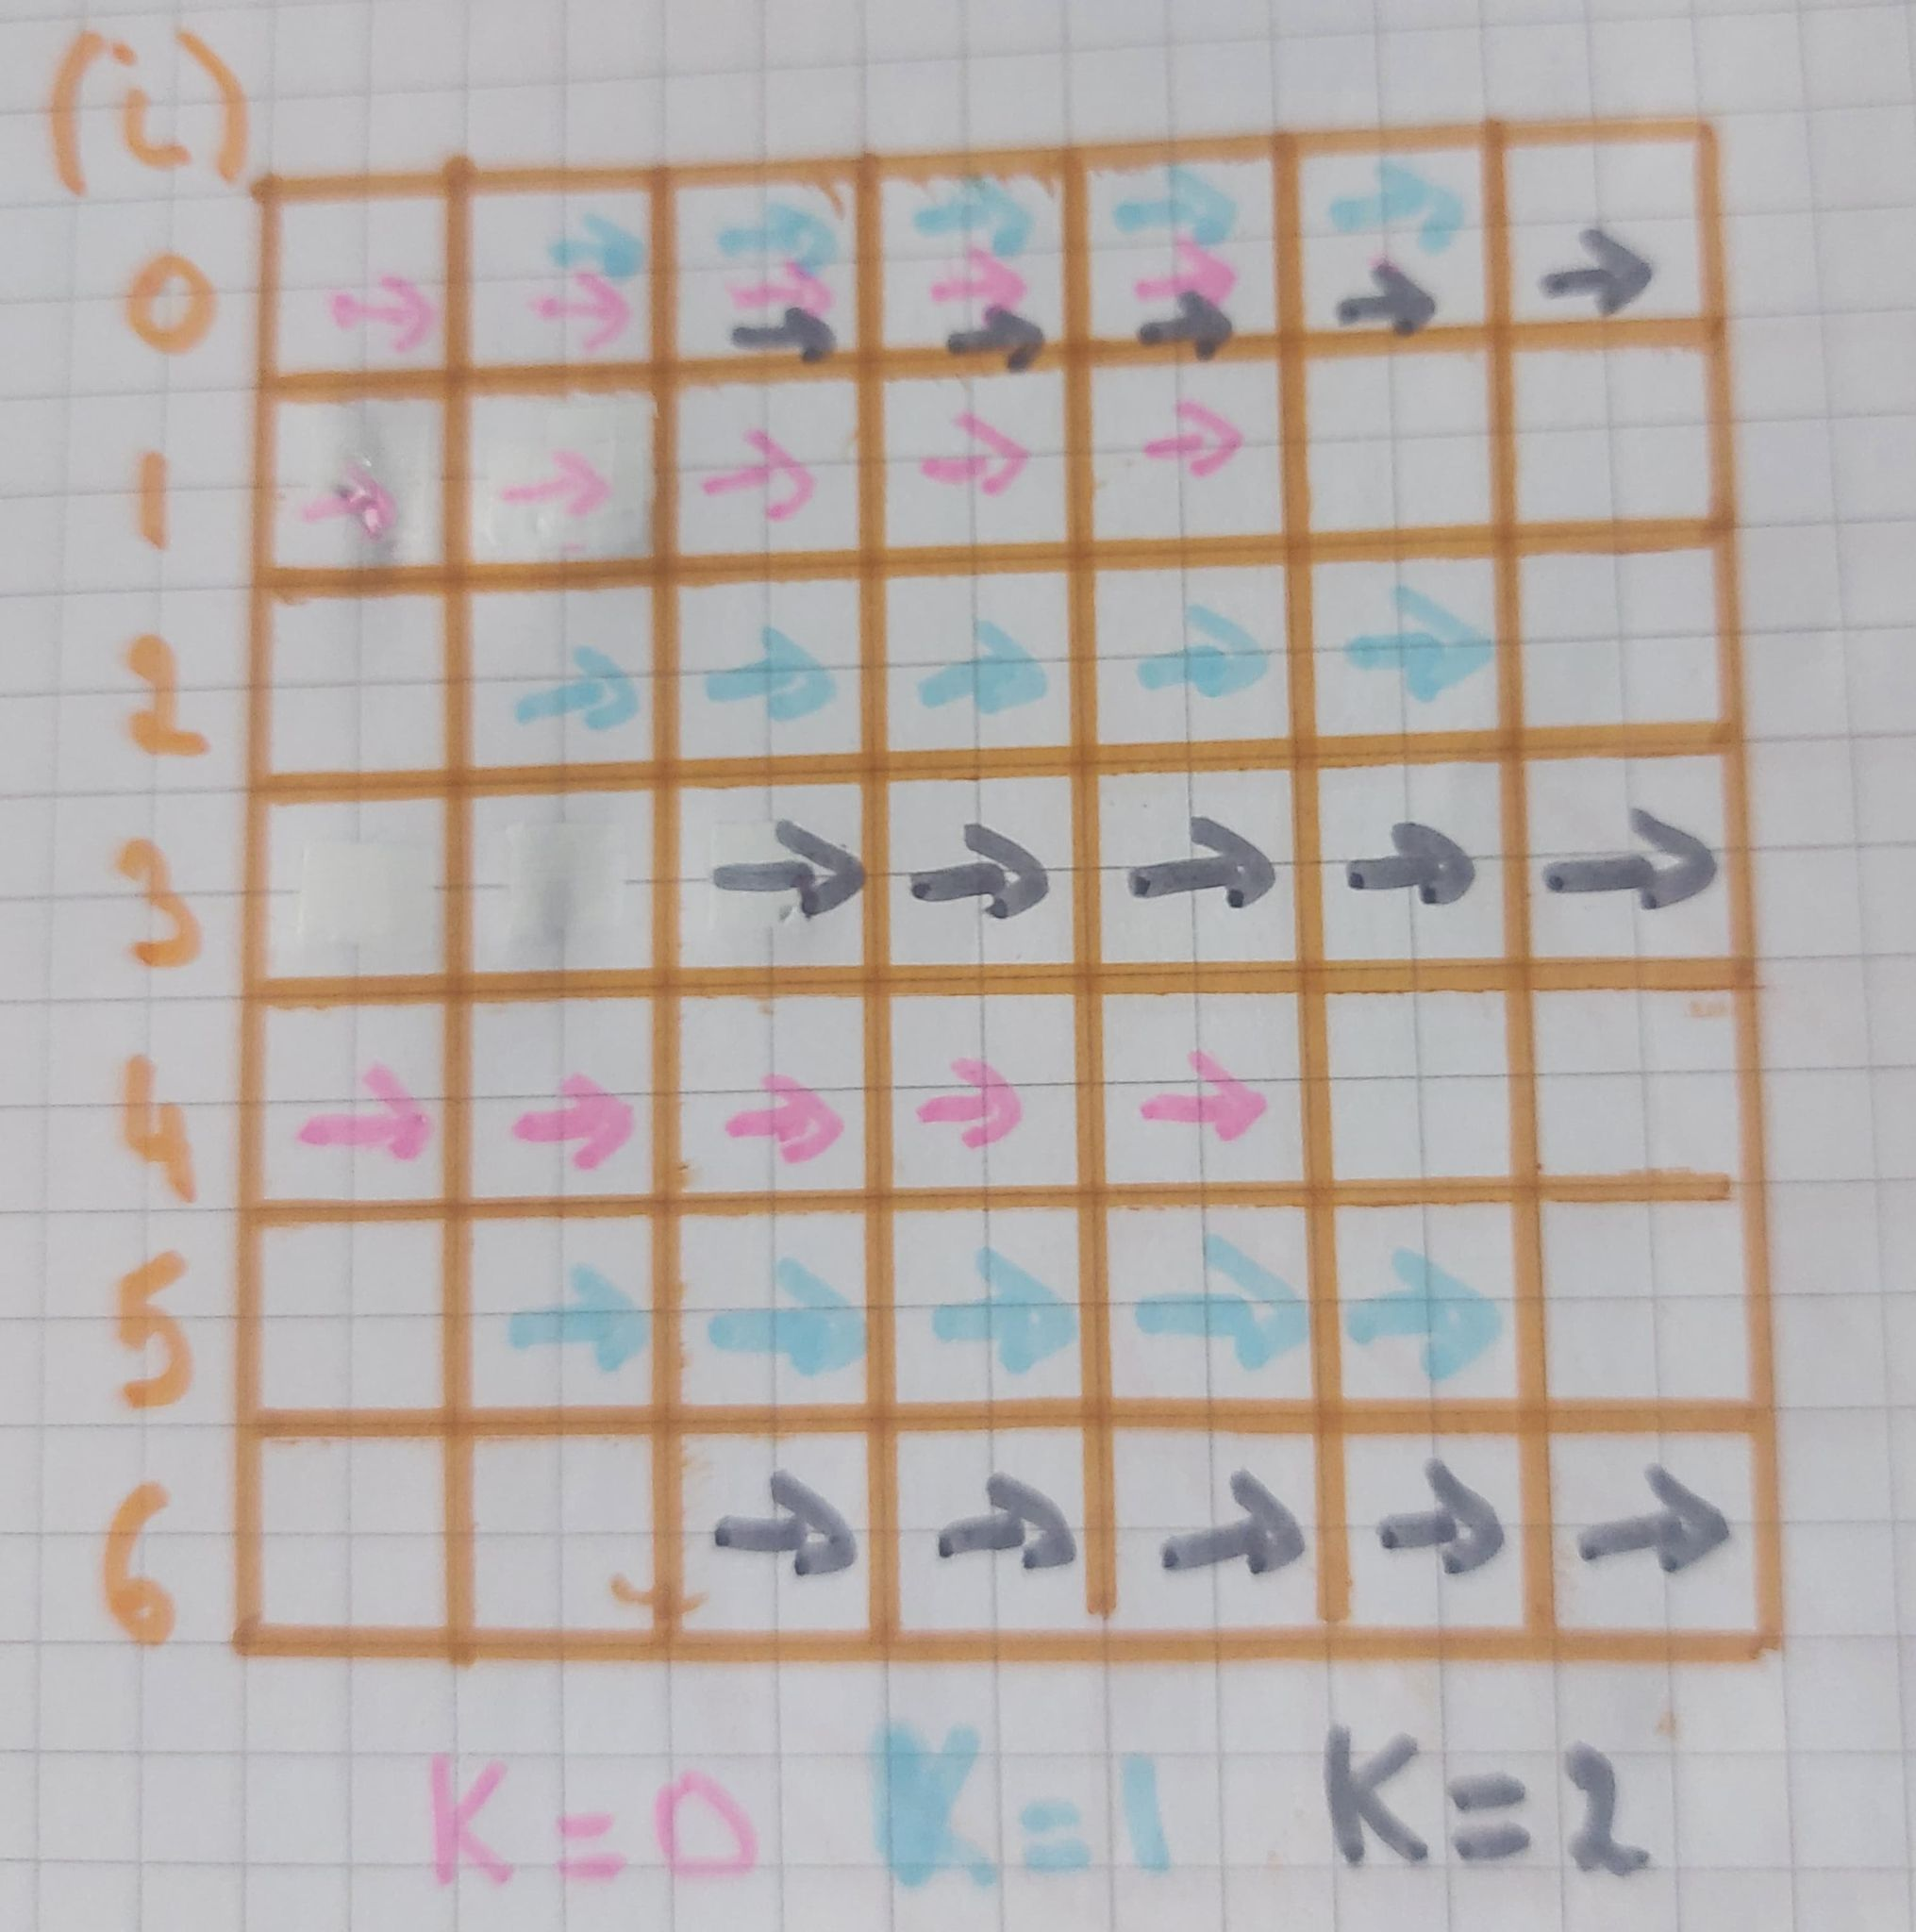
\includegraphics[width=4cm]{./images/horizontale.jpg}\\ 
\end{center} 


\textbf{Idée:}\\
    Cette algorithme pourrait avoir une meillleure complexité mais dans l'idée, elle, nous sert à savoir s'il y a eu un combo horizontale ou non.
\\
\textbf{Implémentation:}\\
Tout d'abord, dans la première boucle nous initialisons la variable "ComboAll" à la plus grande valeur possible du combo et nous la décrementons jusqu'à arriver à 5 qui est le stricte minimum.
La variable "k", nous permet d'avancer d'un pas vers la droite, la variable "i" sert à se déplacer vers le bas et enfin la variable "j" permet de savoir s'il y a bien une suite d'une même couleur.
Voir dessin au dessus.
\newpage

\subsection{Vérification verticale}
\begin{lstlisting}
int verification_verticale( ControleurFive *cf){
    for(int ComboAll = cf->mf->combo ; ComboAll >= 5 ; ComboAll--){
        for(int k = 0; k < cf->mf->avancer_tableau_verticale; k++){
            for(int i = 0; i < cf->mf->largeur; i++){
                for(int j = 1; j< cf->mf->typeSymboles+1; j++){
                }
                // Avec tous les if
            }
        }
    }
}
\end{lstlisting}
\begin{center}
    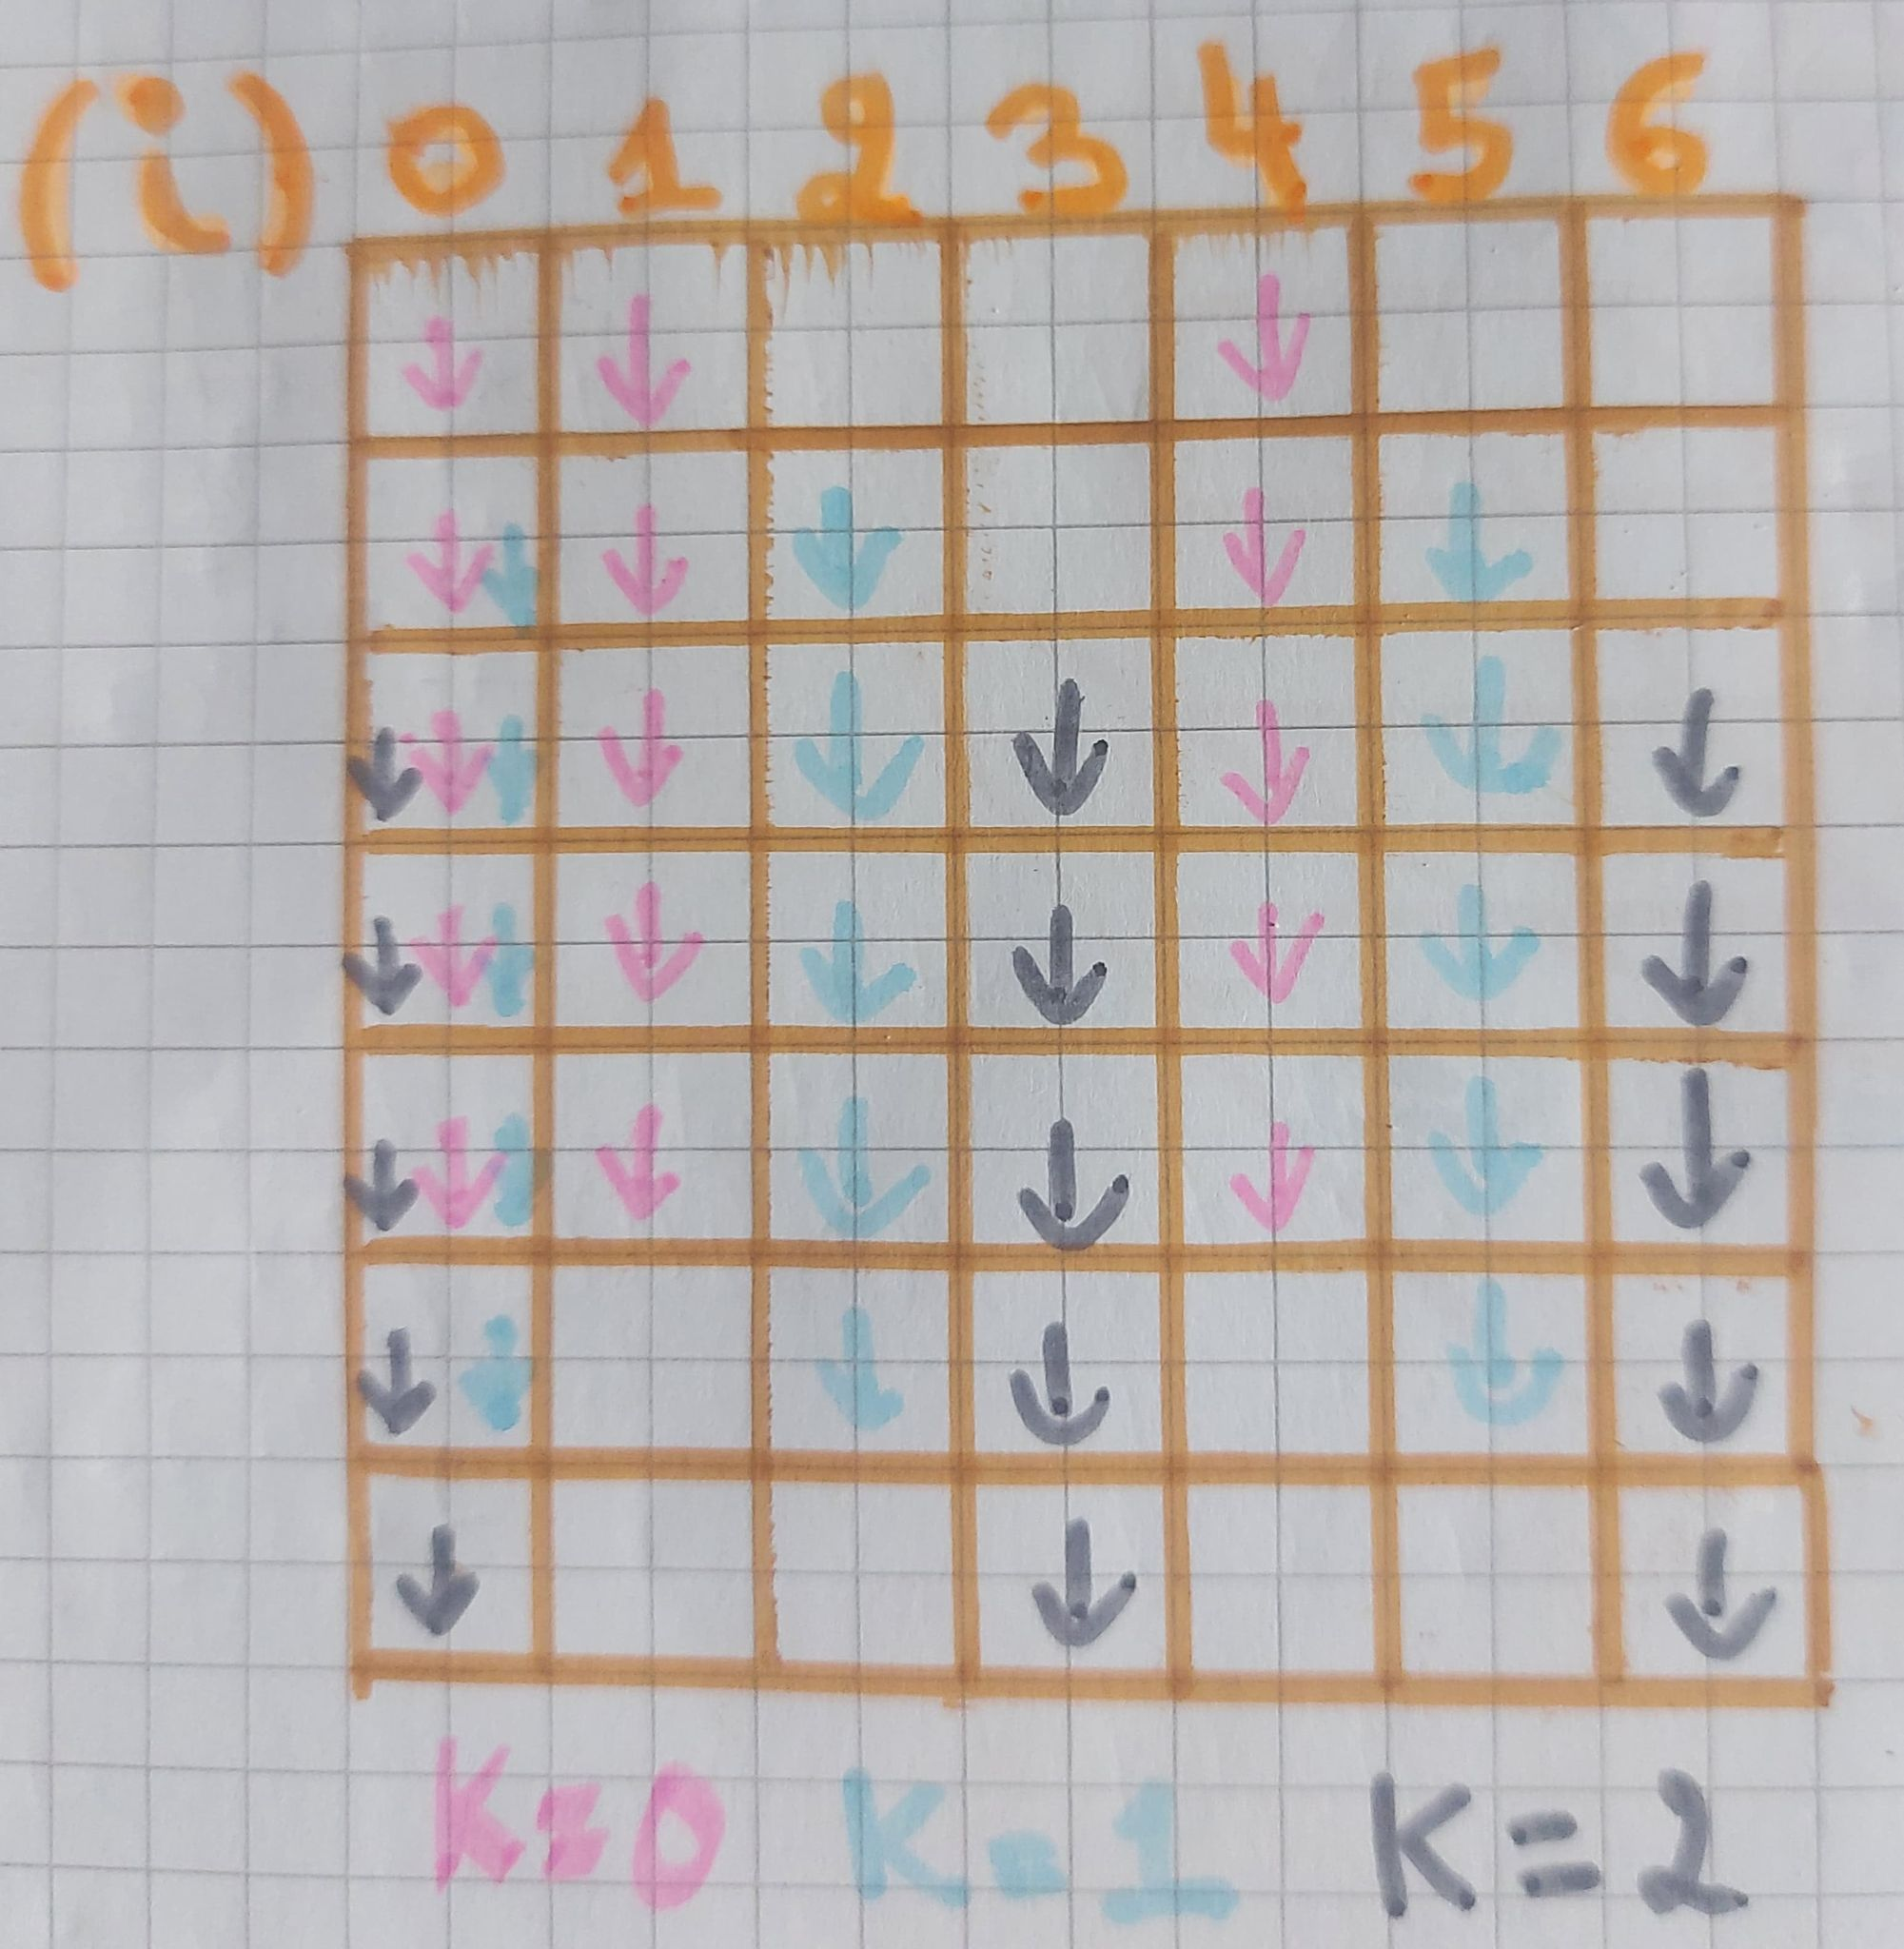
\includegraphics[width=4cm]{./images/verticale.jpg}\\ 
\end{center} 


\textbf{Idée:}\\
Cette algorithme pourrait avoir une meillleure complexité mais dans l'idée, elle, nous sert à savoir s'il y a eu un combo verticale ou non.
\\
\textbf{Implémentation:}\\
Tout d'abord, dans la première boucle nous initialisons la variable "ComboAll" à la plus grande valeur possible du combo et nous la décrementons jusqu'à arriver à 5 qui est le stricte minimum.
La variable "k", nous permet d'avancer d'un pas vers le bas, la variable "i" nous sert à se déplacer vers la droite et enfin la variable "j" permet de savoir s'il y a bien une suite d'une même couleur.
Voir dessin au dessus.
\subsection{Vérification croissante}
\begin{lstlisting}
int oblique_croissant1(ControleurFive *cf){
    for(int ComboAll = cf->mf->combo; ComboAll >= 5; ComboAll--){
        for(int i = 0; i < cf->mf->largeur - 3; i++){ 
            for(int k = 0; k < cf->mf->avancer_tableau_oblique; k++){
                for(int j = 1; j< cf->mf->typeSymboles +1; j++){
                    //Avec tous les if
                }
            }
        }
    }
}
int oblique_croissant2(ControleurFive *cf){
    for(int ComboAll = cf->mf->combo; ComboAll >= 5; ComboAll--){
        for(int i = 4;i < cf->mf->hauteur - 1; i++){
            for(int k = 0; k < cf->mf->avancer_tableau_oblique - 1; k++){
                for(int j = 1; j< cf->mf->typeSymboles + 1; j++){
                    //Avec tous les if
                }
            }
        }
    }
}
\end{lstlisting}
\begin{figure}[!h]
    \centering
    \begin{subfigure}[]{}
        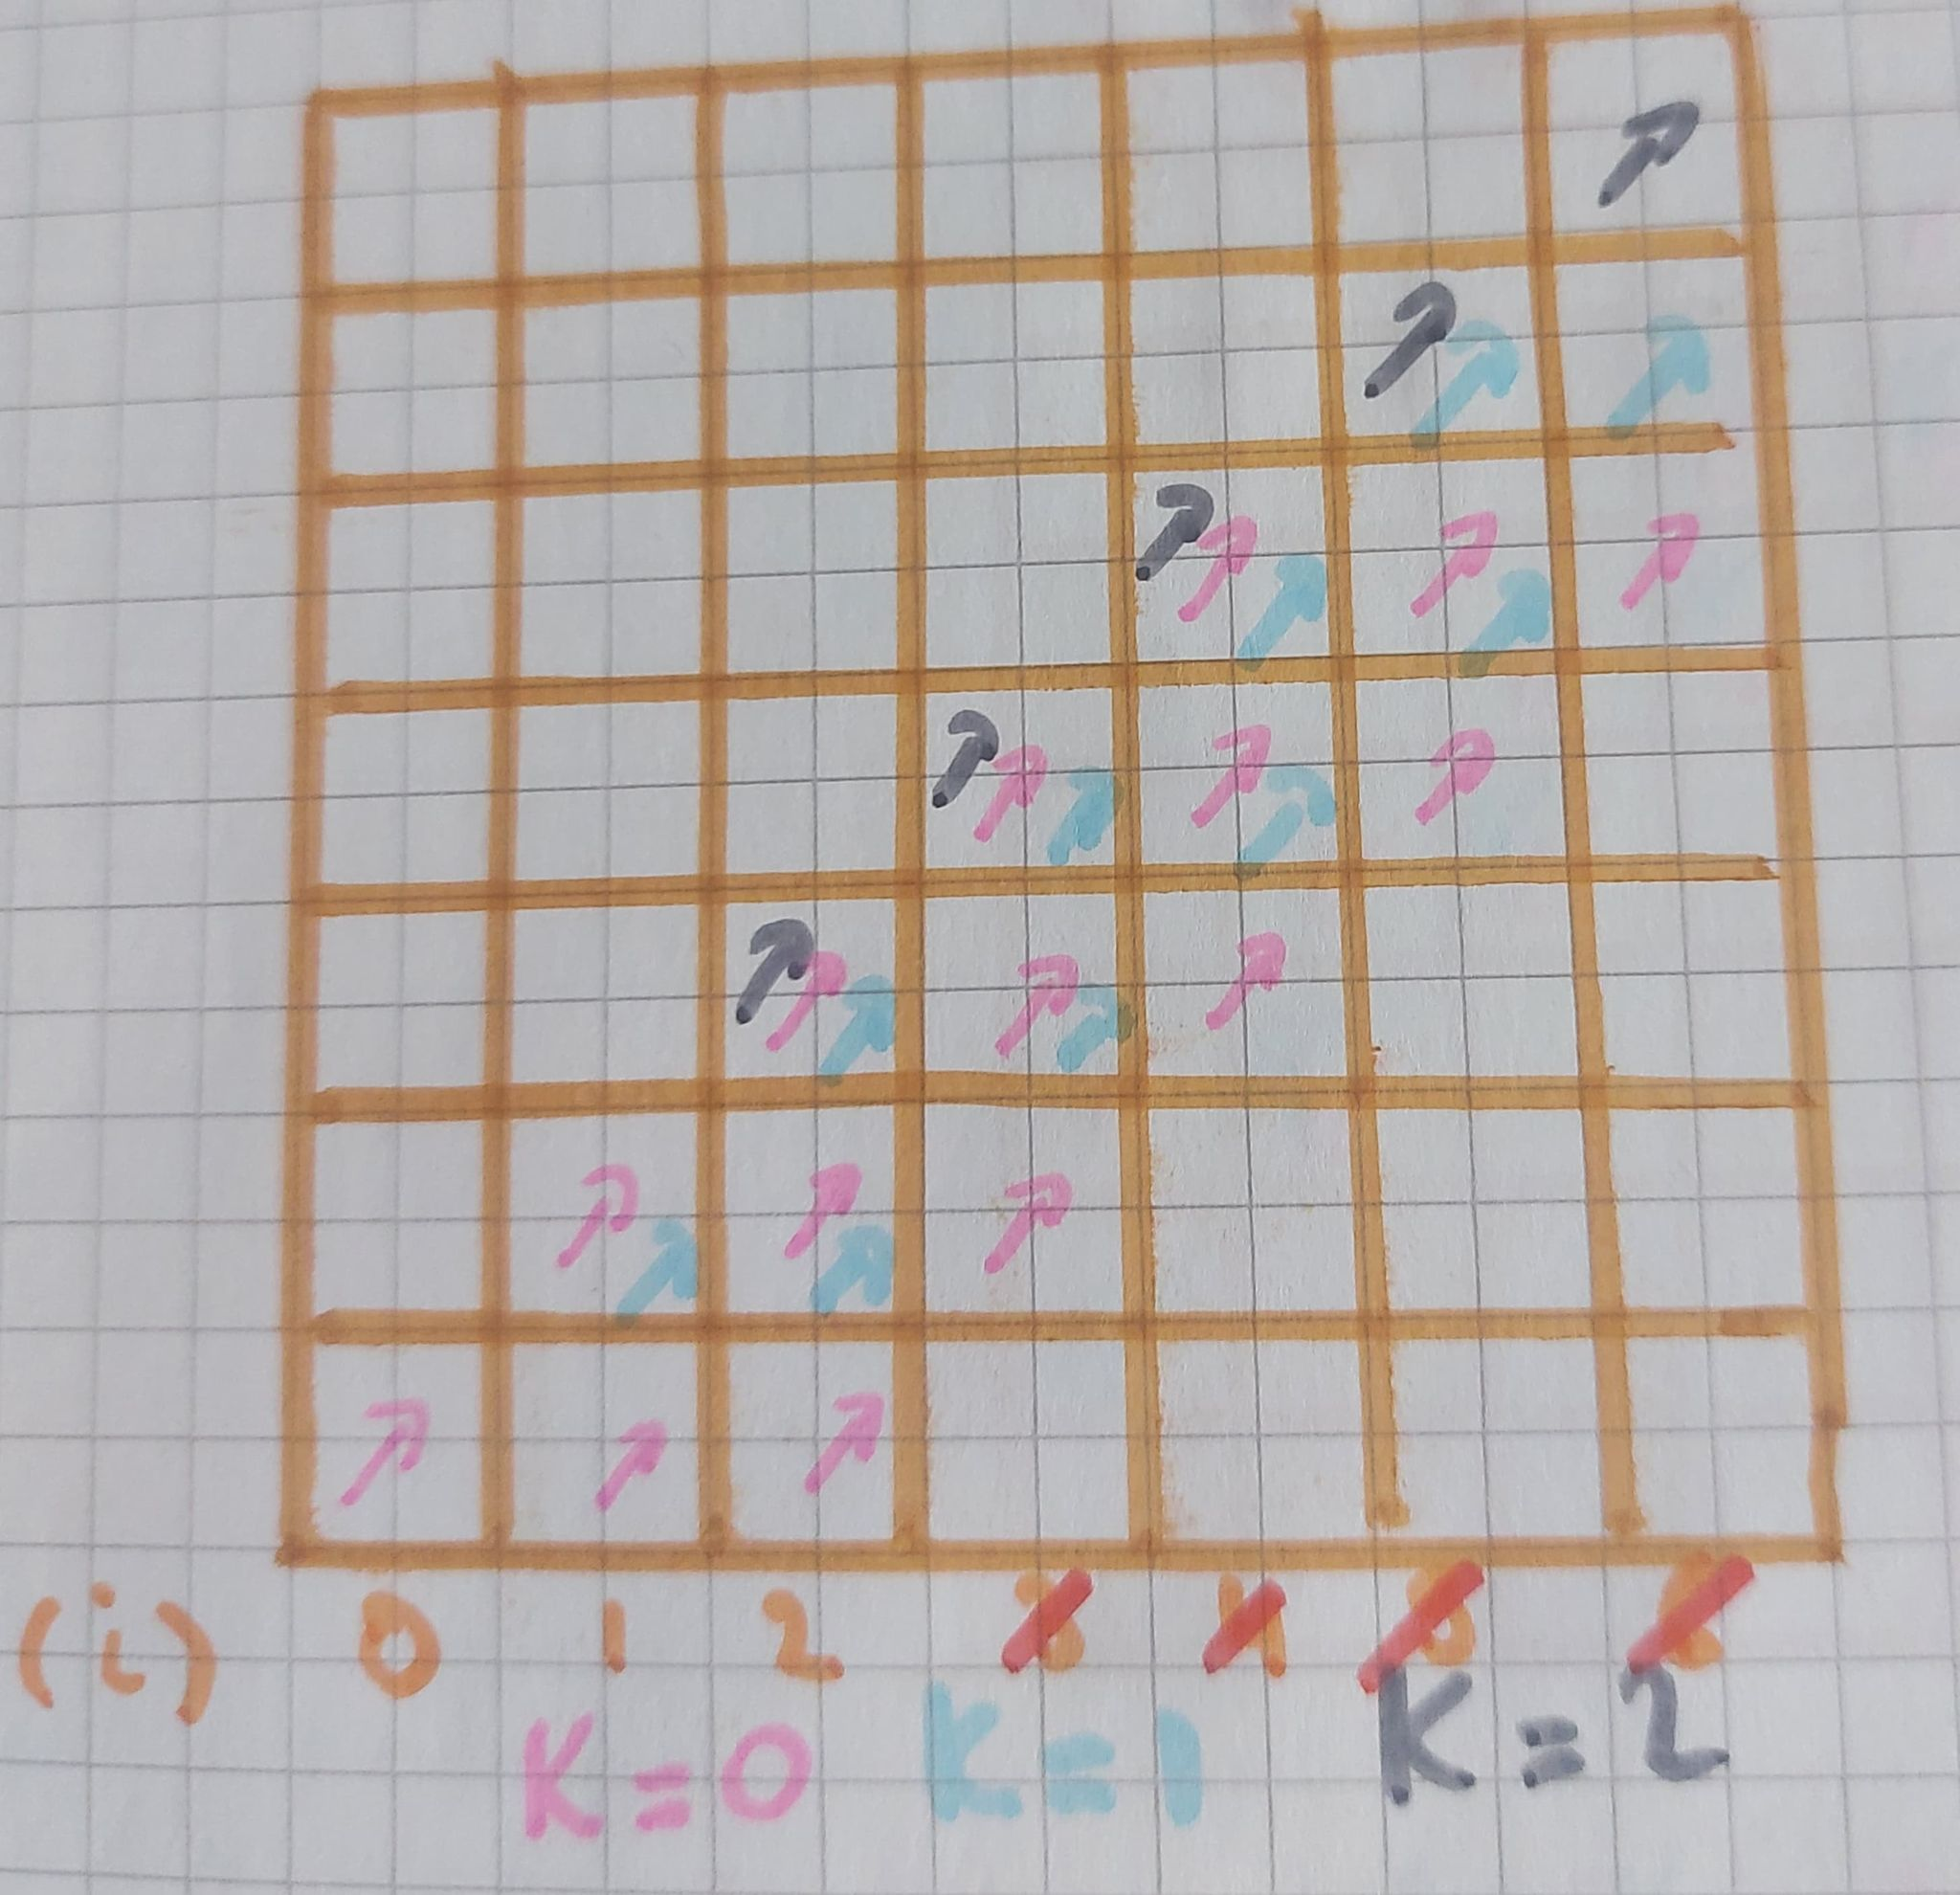
\includegraphics[width=4cm]{./images/croissant1.jpg}
    \end{subfigure}
    \begin{subfigure}[]{}
        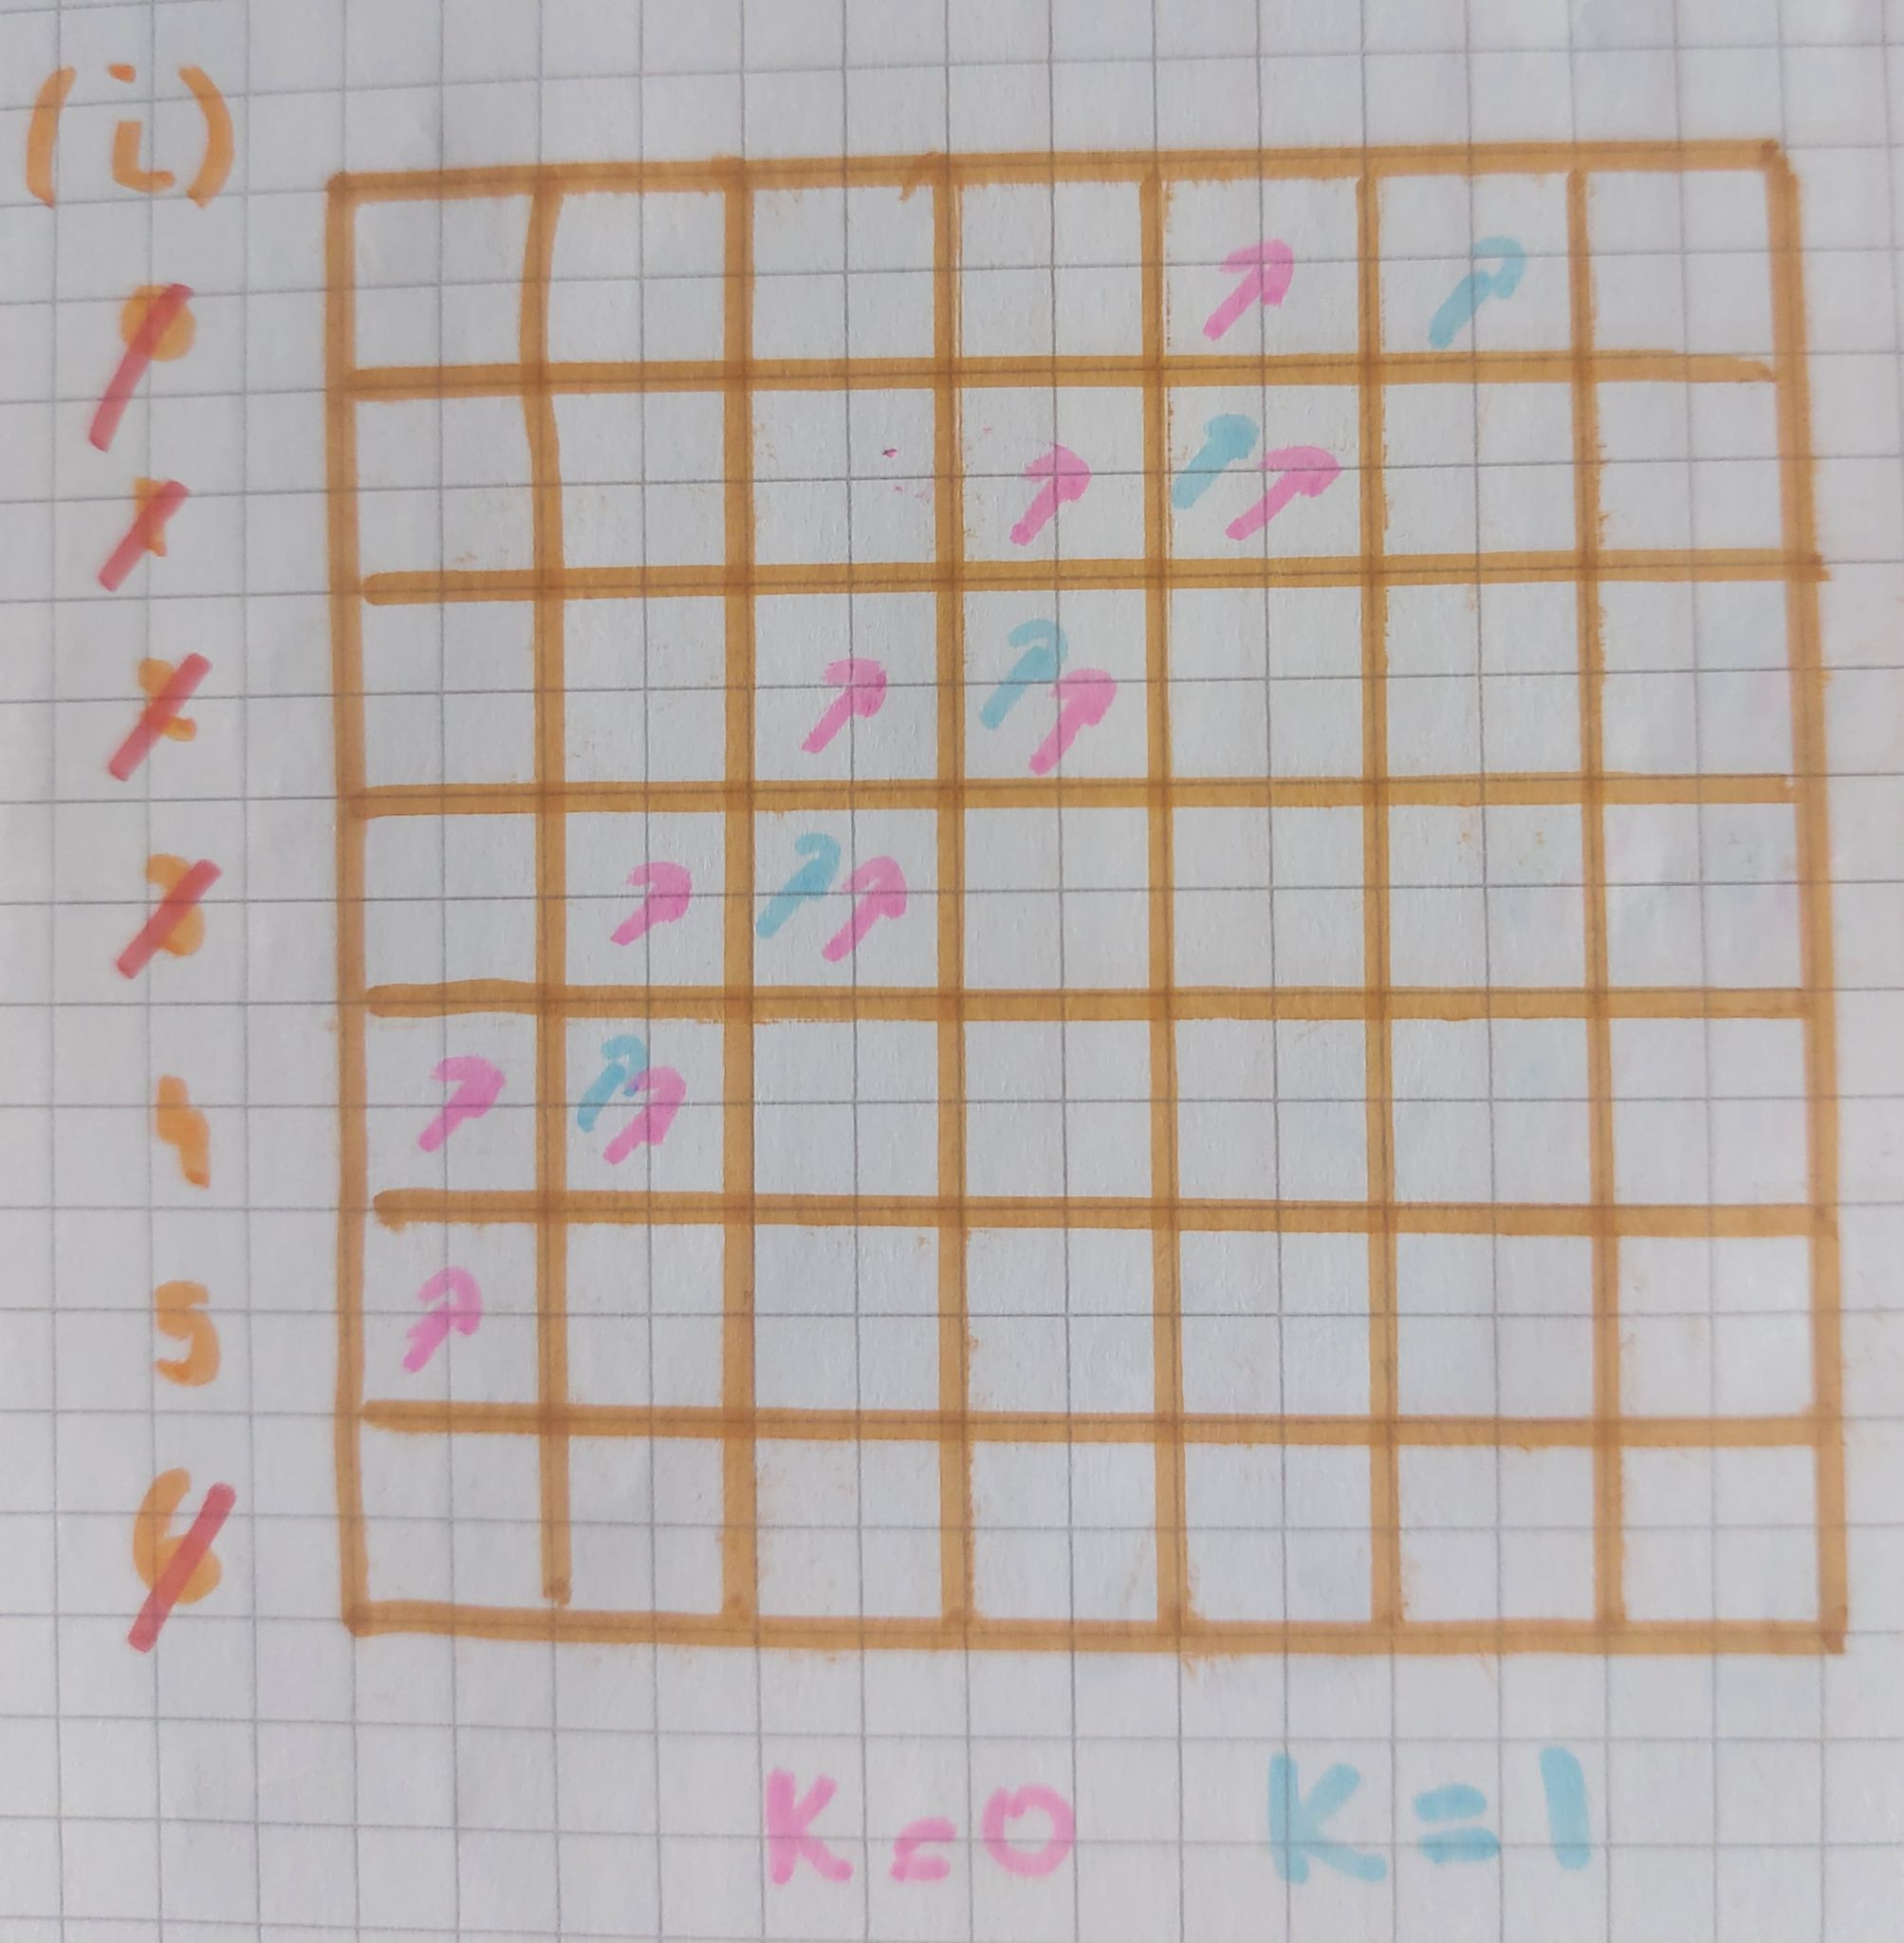
\includegraphics[width=4cm]{./images/croissant2.jpg}
    \end{subfigure}
\end{figure}
    
\textbf{Idée:}\\
Cette algorithme pourrait avoir une meillleure complexité mais dans l'idée, elle, nous sert à savoir s'il y a eu un combo croissant ou non.
\\
\textbf{Implémentation:}\\
Tout d'abord, dans la première boucle nous initialisons la variable "ComboAll" à la plus grande valeur possible du combo et nous la décrementons jusqu'à arriver à 5 qui est le stricte minimum.
La variable "k", nous permet d'avancer d'un pas oblique croissant, la variable "i" nous permet de se déplacer vers le haut pour 'croissant1' $\equiv$ (image a) et la même variable permet de se déplacer vers la droite pour 'croissant2' $\equiv$ (image b).Et enfin la variable "j" permet de savoir s'il y a bien une suite d'une même couleur.
Voir les deux dessins au dessus.

\subsection{Vérification décroissante}
\begin{lstlisting}
int oblique_decroissant1(ControleurFive *cf){
    for(int ComboAll = cf->mf->combo; ComboAll >= 5; ComboAll--){
        for(int k = 0; k < cf->mf->avancer_tableau_horizontale; k++){
            for(int i = 0; i < cf->mf->hauteur - 4; i++){
                for(int j = 1; j< cf->mf->typeSymboles + 1; j++){
                    //Avec tous les if
                }
            }
        }
    }
}
int oblique_decroissant2(ControleurFive *cf){
   for(int ComboAll = cf->mf->combo; ComboAll >= 5; ComboAll--){
        for(int i = 0;i < cf->mf->largeur - 5; i++){
            for(int k = 0; k < cf->mf->avancer_tableau_horizontale - 1; k++){
                for(int j = 1; j< cf->mf->typeSymboles+1; j++){
                    //Avec tous les if
                }
            }
        }
    }
}
\end{lstlisting}

\begin{figure}[!h]
    \centering
    \begin{subfigure}[]{}
        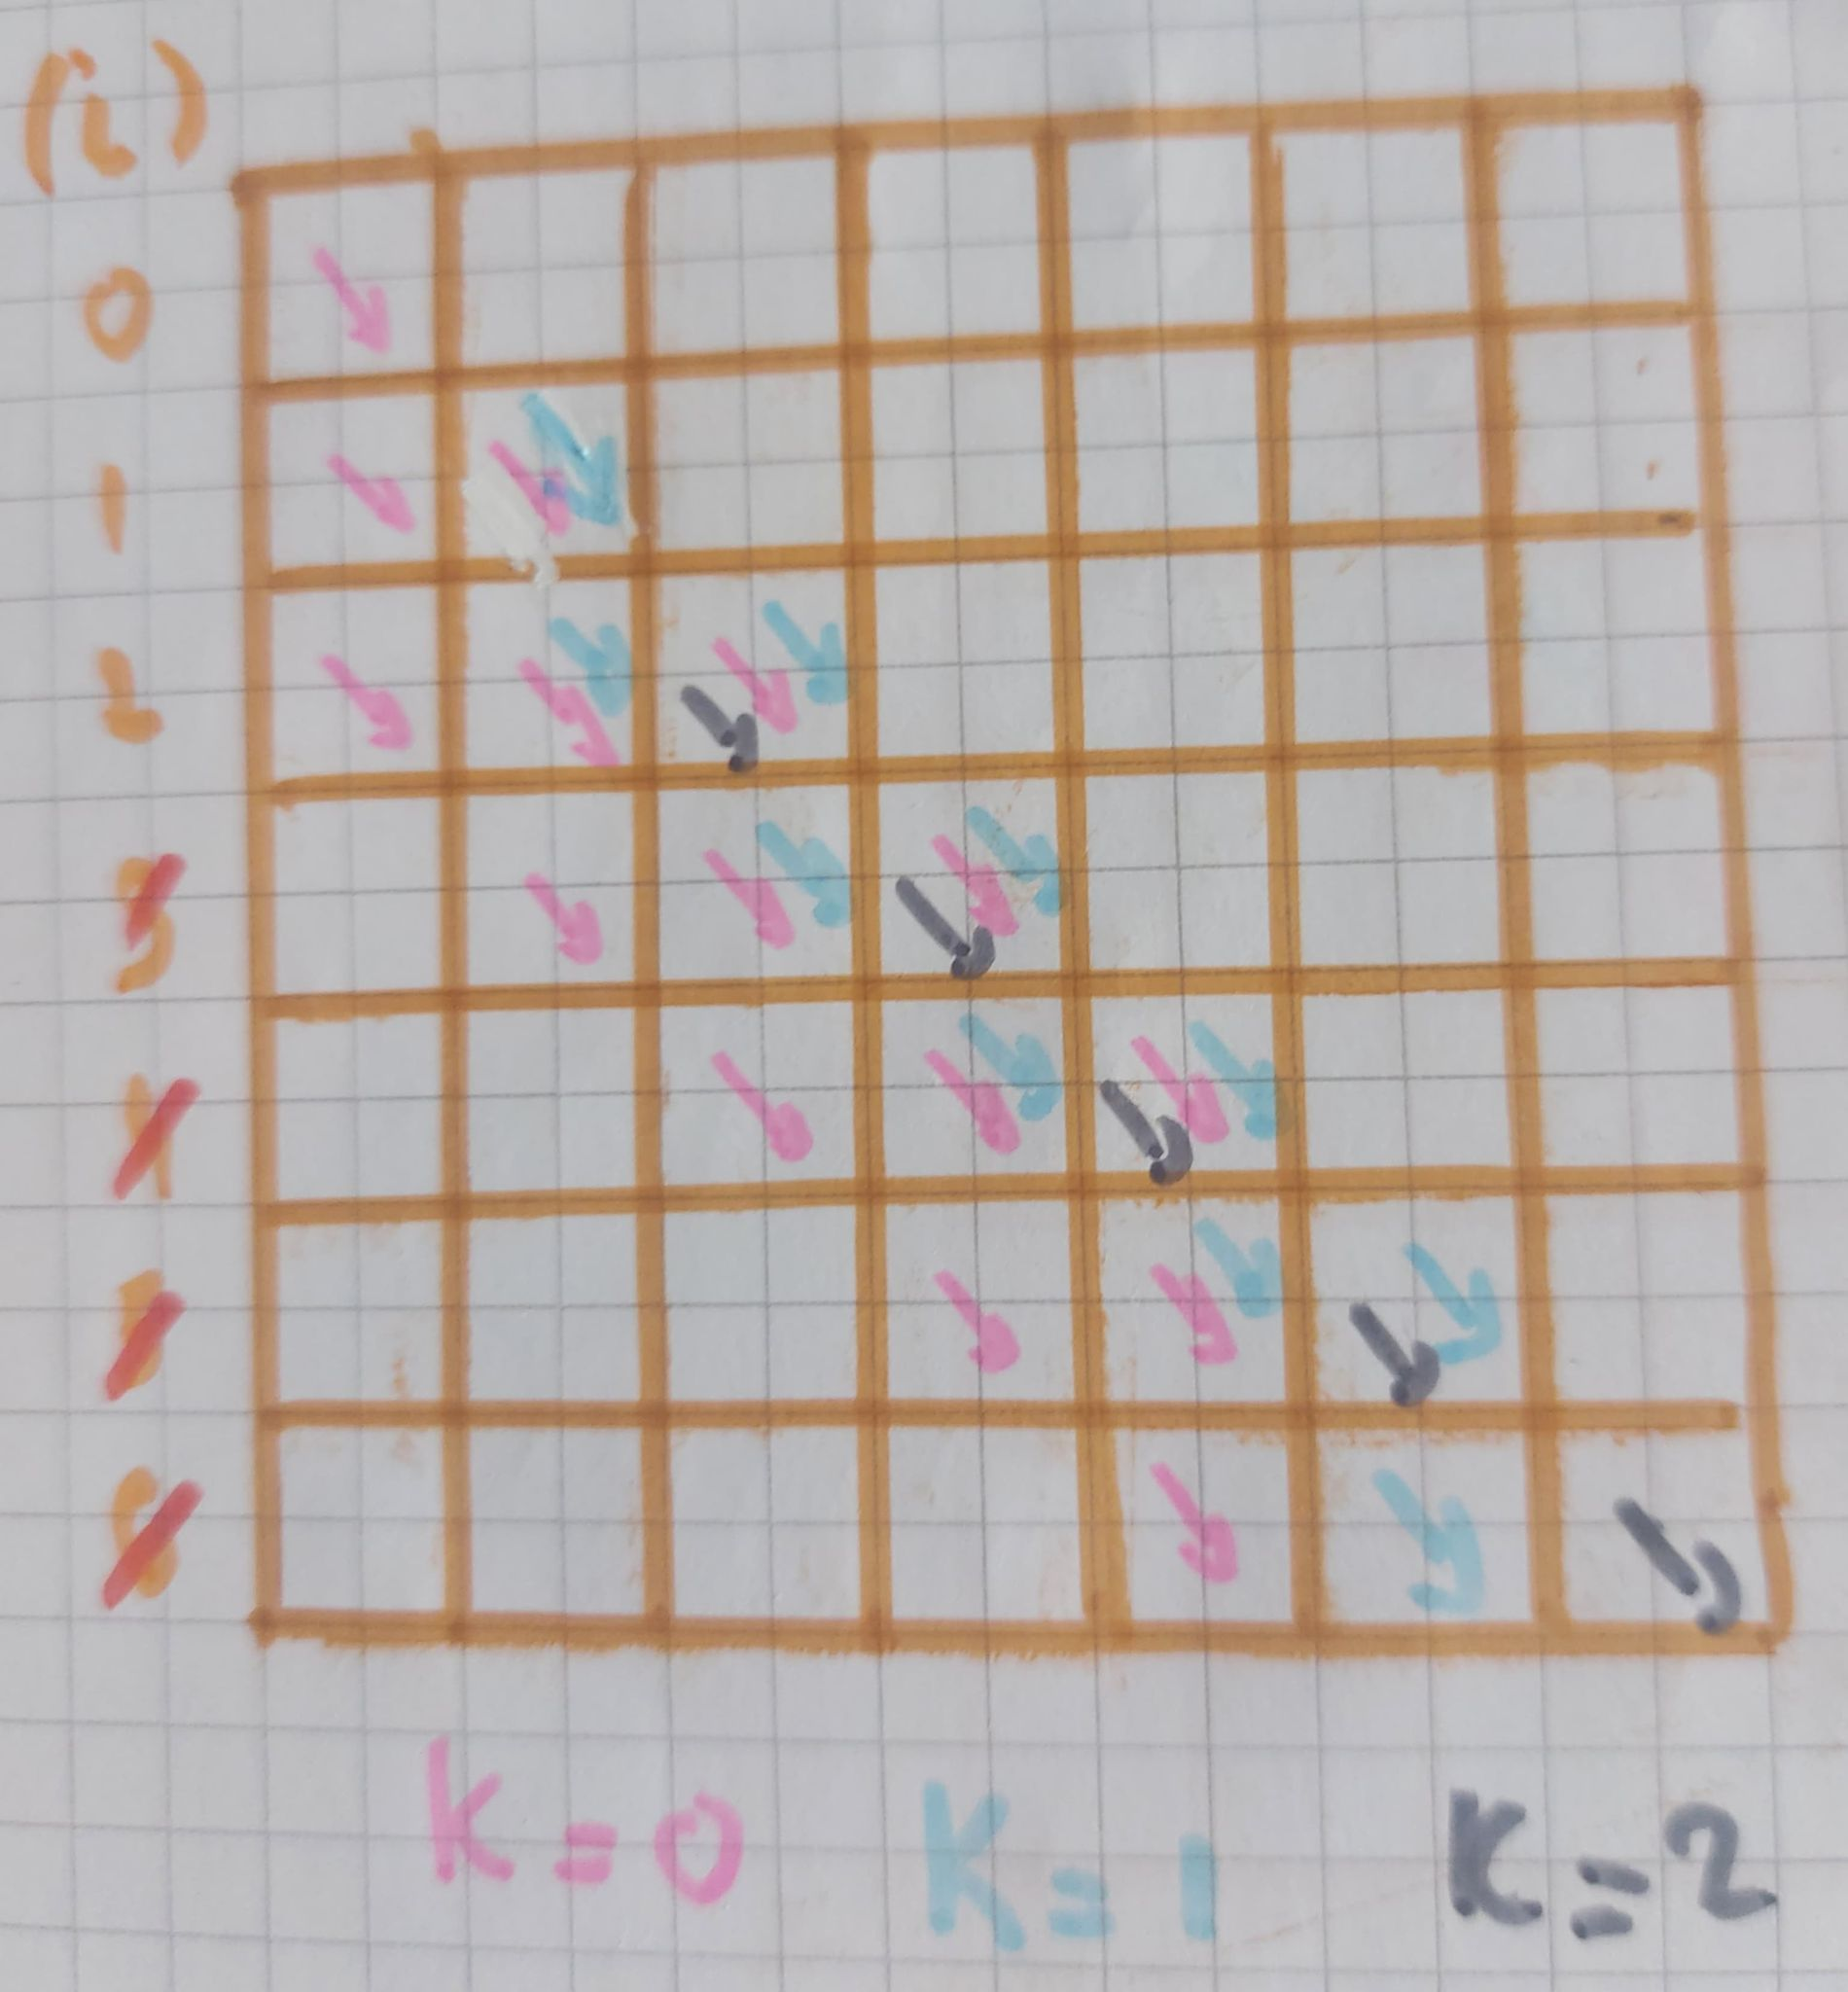
\includegraphics[width=4cm]{./images/decroissant1.jpg}
    \end{subfigure}
    \begin{subfigure}[]{}
        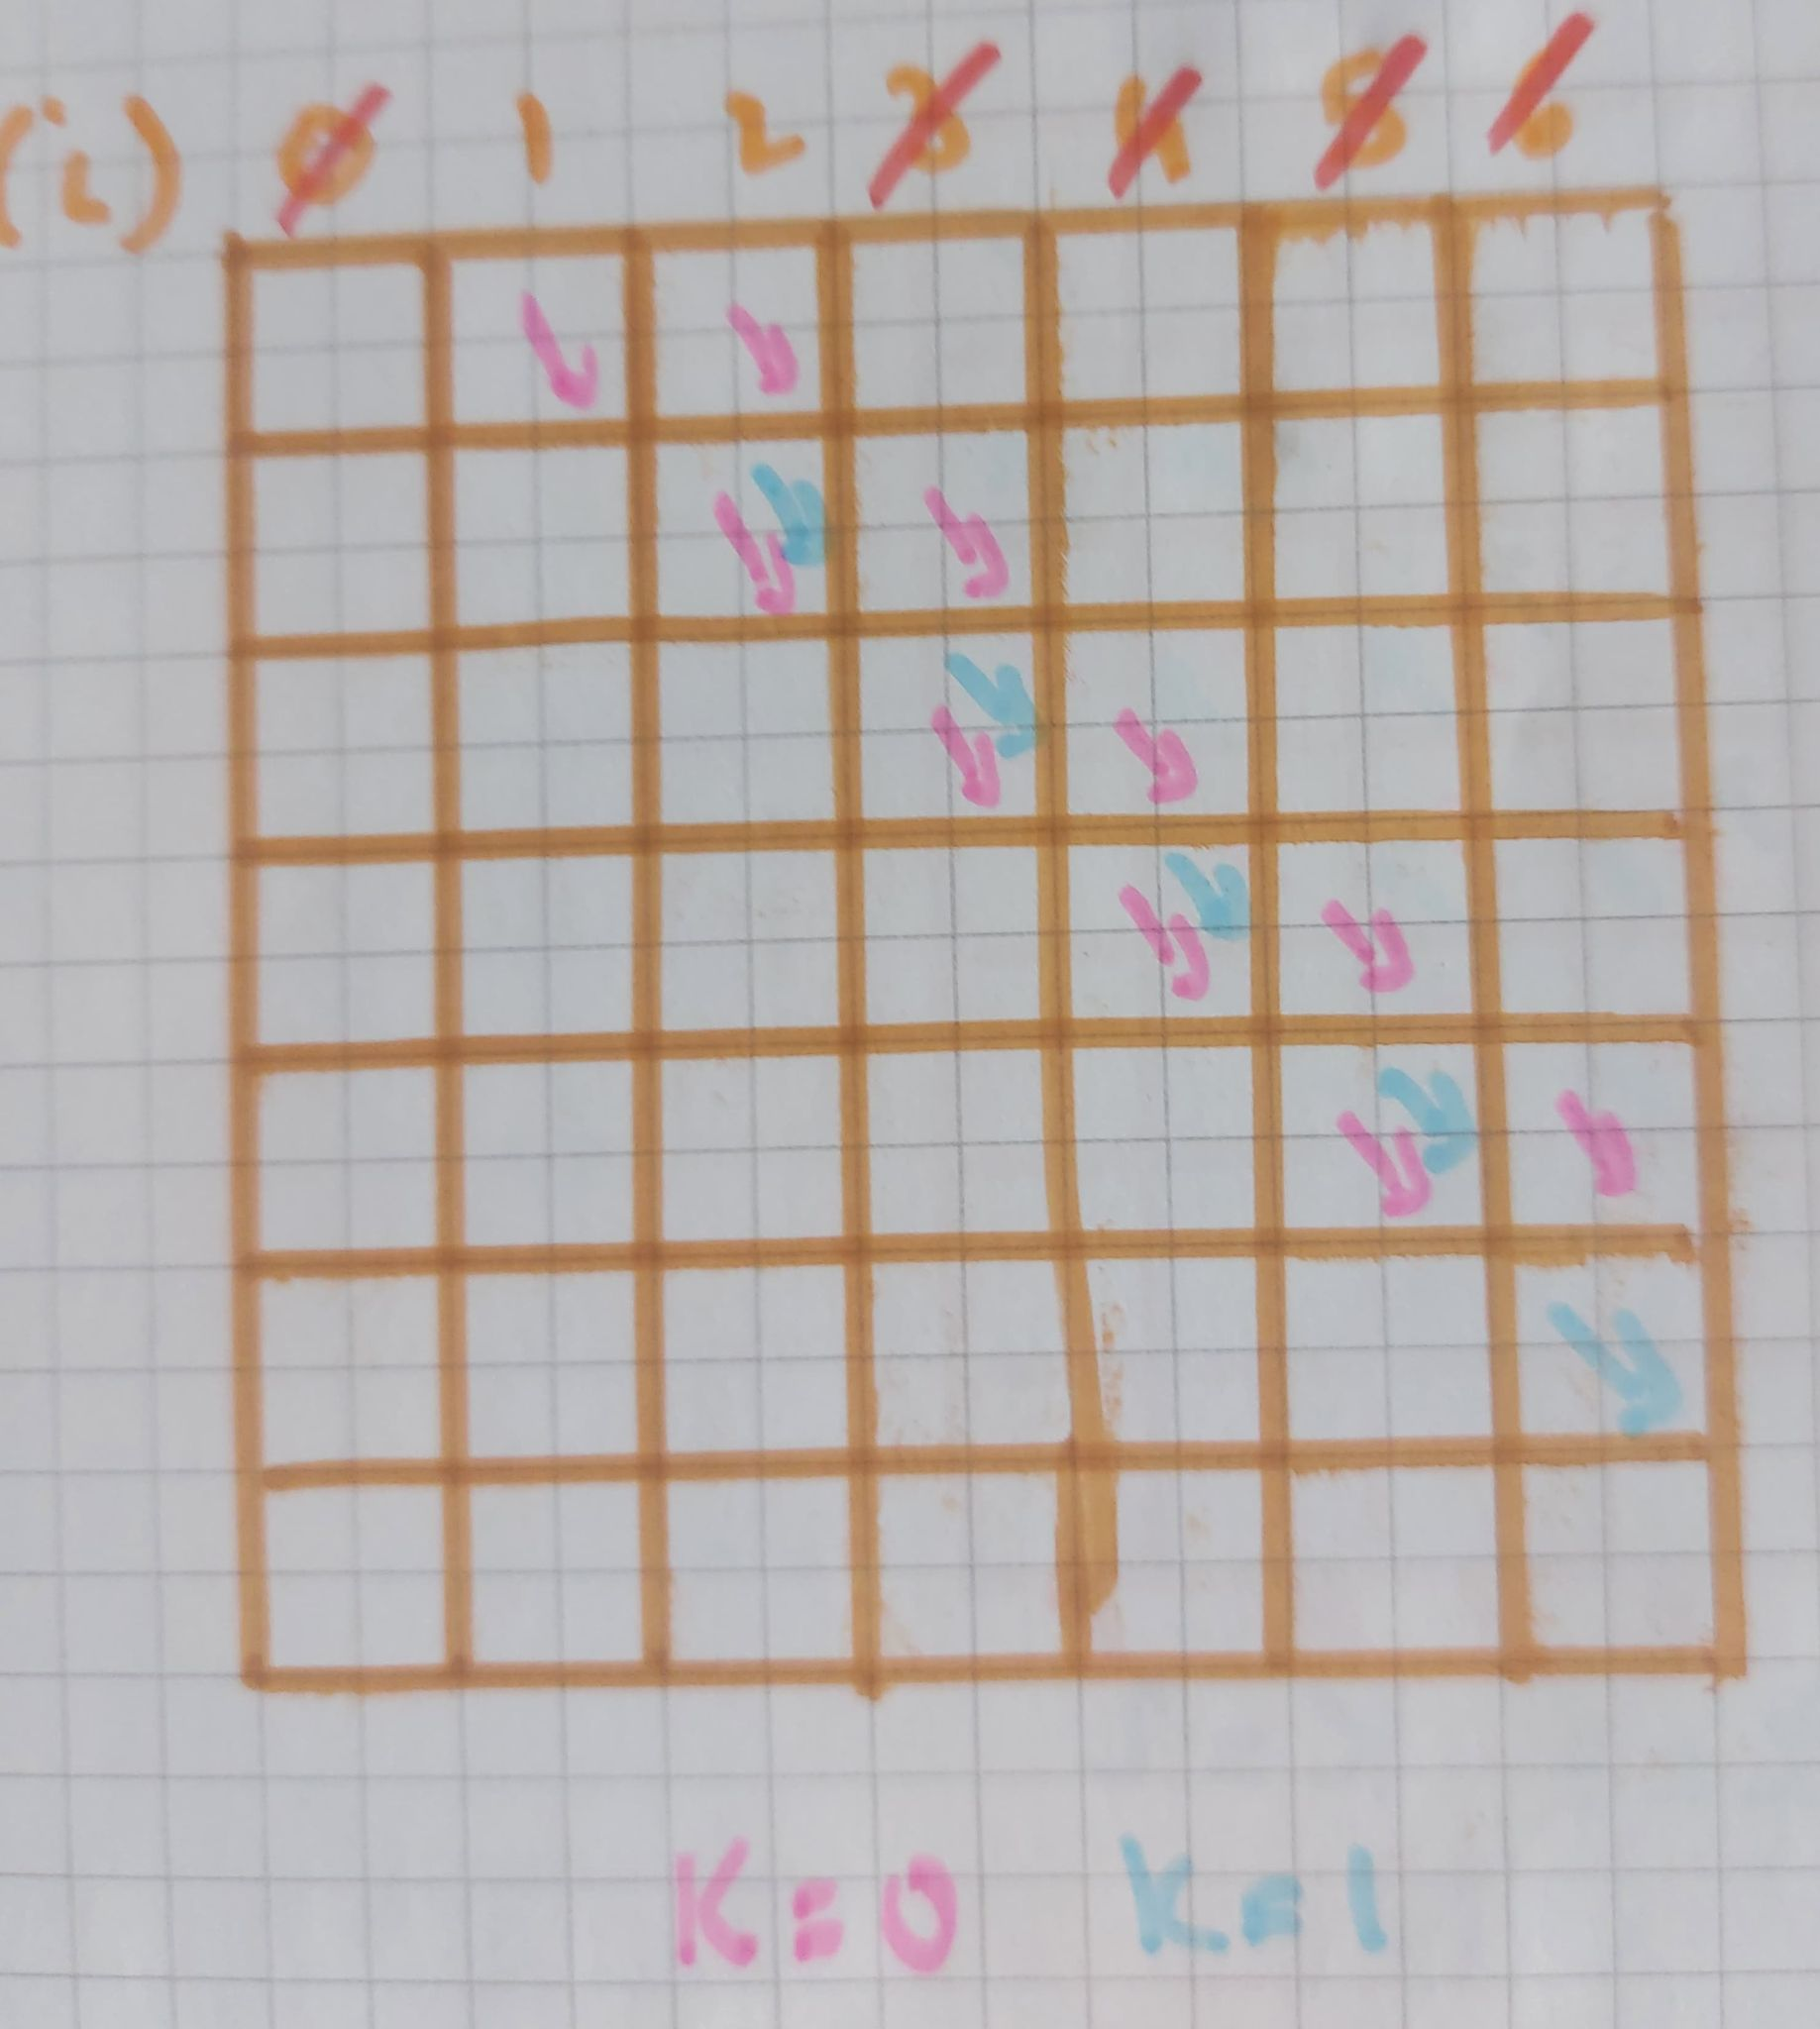
\includegraphics[width=4cm]{./images/decroissant2.jpg}
    \end{subfigure}
\end{figure}
    
\textbf{Idée:}\\
Cette algorithme pourrait avoir une meillleure complexité mais dans l'idée, elle, nous sert à savoir s'il y a eu un combo decroissant ou non.
\\
\textbf{Implémentation:}\\
Tout d'abord, dans la première boucle nous initialisons la variable "ComboAll" à la plus grande valeur possible du combo et nous la décrementons jusqu'à arriver à 5 qui est le stricte minimum pour un combo.
La variable "k", nous permet d'avancer d'un pas oblique décroissant, la variable "i" nous permet de se déplacer vers le bas pour 'décroissant1' $\equiv$ (image a) et la même variable permet de se déplacer vers la droite pour 'décroissant2' $\equiv$ (image b).Et enfin la variable "j" permet de savoir s'il y a bien une suite d'une même couleur.
Voir les deux dessins au dessus.

\subsection{Génération image aléatoire}
\begin{lstlisting}
int generation_image_aleatoire(ModeleFive *mf){
   int compteur = 0;
   for (int i = 0; i < mf->hauteur; i++){
      for (int j = 0; j < mf->largeur; j++){
         position_case_blanche(mf, i, j, 0);
         if(mf->grille[i][j] == 0){
            compteur += 1;
            position_case_blanche(mf, i, j, compteur);  
         }
      }
   }
   if(compteur != 0){
      srand(time(NULL));
      int a = rand () % compteur;
      for (int i = 0; i < mf->hauteur; i++){
         for (int j = 0; j < mf->largeur; j++){
            if(mf->aleatoire[i][j] == a + 1){ 
               compteur = (i * mf->largeur) + j;
            }
         }
      }
   }
return compteur;
}
\end{lstlisting}
\textbf{Idée:}\\
    Cette algorithme semble avoir une bonne complexité 
\\
\textbf{Implémentation:}\\
Tout d'abord, un compteur est incrémenté quand il trouve une case blanche et stocke ses coordonnées dans la fonction position\_case\_blanche. Ensuite, un nombre aléatoire va être généré et nous allons utiliser l'opérande modulo pour avoir un nombre compris entre 0 et le compteur - 1.
Par après, on retourne la position d'une des cases blanches de la grille.

\section{Profiling et analyse de performance du code}
Pour le profiling, nous avons utilisé gprof qui nous a permis de calculer la performance de notre projet. Nous avons pu constater que certaines fonctions prennaient plus de temps que d'autres. 
Sur la photo ci-dessous , nous pouvons y voir que la fonction decroissant1 a pris le plus du temps vu la complexité de cette fonction.\\
\begin{center}
    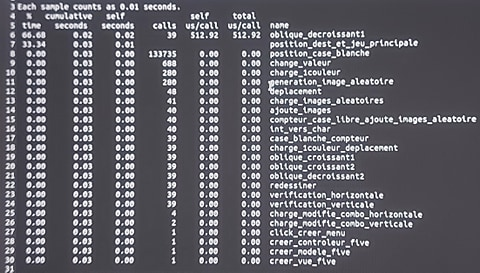
\includegraphics[width=7cm]{./images/gprof.jpg}
\end{center}

\textbf{ModeleFive:}\\ 
Constitue la structure complète, elle a une taille de 2492 bytes car (13 int * 4 bytes) + 2 * ( 20 hauteur * 15 largeur * 4 bytes) + ( 10 * 4 bytes)
\\ \\

\textbf{VueFive:}\\
Pour le niveau 0 : elle a une taille de 460 bytes car (49 * 8 bytes) + 2*(3 * 8 bytes) + 8 + ( 3 * 4)
\newline
Pour le niveau 1 : elle a une taille de 716 bytes car (81 * 8 bytes) + 2*(3 * 8 bytes) + 8 + ( 3 * 4)
\newline
Pour le niveau 2 : elle a une taille de 2484 bytes car (300 * 8 bytes) + 2*(7 * 8 bytes) + 8 + ( 7 * 4)
\\ \\
\textbf{ControleurFive:}\\
Pour le niveau 0 : elle a une taille de $\pm$420 bytes car (49 * 8 bytes) + (nombre caractere fichier * 1 bytes) + 8 bytes + ( 5 * 4 bytes)
\newline
Pour le niveau 1 : elle a une taille de $\pm$676 bytes car (81 * 8 bytes) + (nombre caractere fichier * 1 bytes) + 8 bytes + ( 5 * 4 bytes)
\newline
Pour le niveau 2 : elle a une taille de $\pm$2428 bytes car (300 * 8 bytes) + (nombre caractere fichier * 1 bytes) + 8 bytes + ( 5 * 4 bytes)

\section{L’interface graphique du jeu}
\subsection{Vue générale du jeu}
Le jeu Five or more est composé de 3 niveaux:
\newline
a)Le mode facile composé d'une grille 7x7 avec 3 boutons informations et tous ses compléments
\newline
b)Le mode moyen composé d'une grille 9x9 avec 3 boutons informations et tous ses compléments
\newline
c)Le mode difficile composé d'une grille 20x15 avec 7 boutons informations et tous ses compléments
\newline
\begin{figure}[!h]
    \centering
    \begin{subfigure}[]{}
        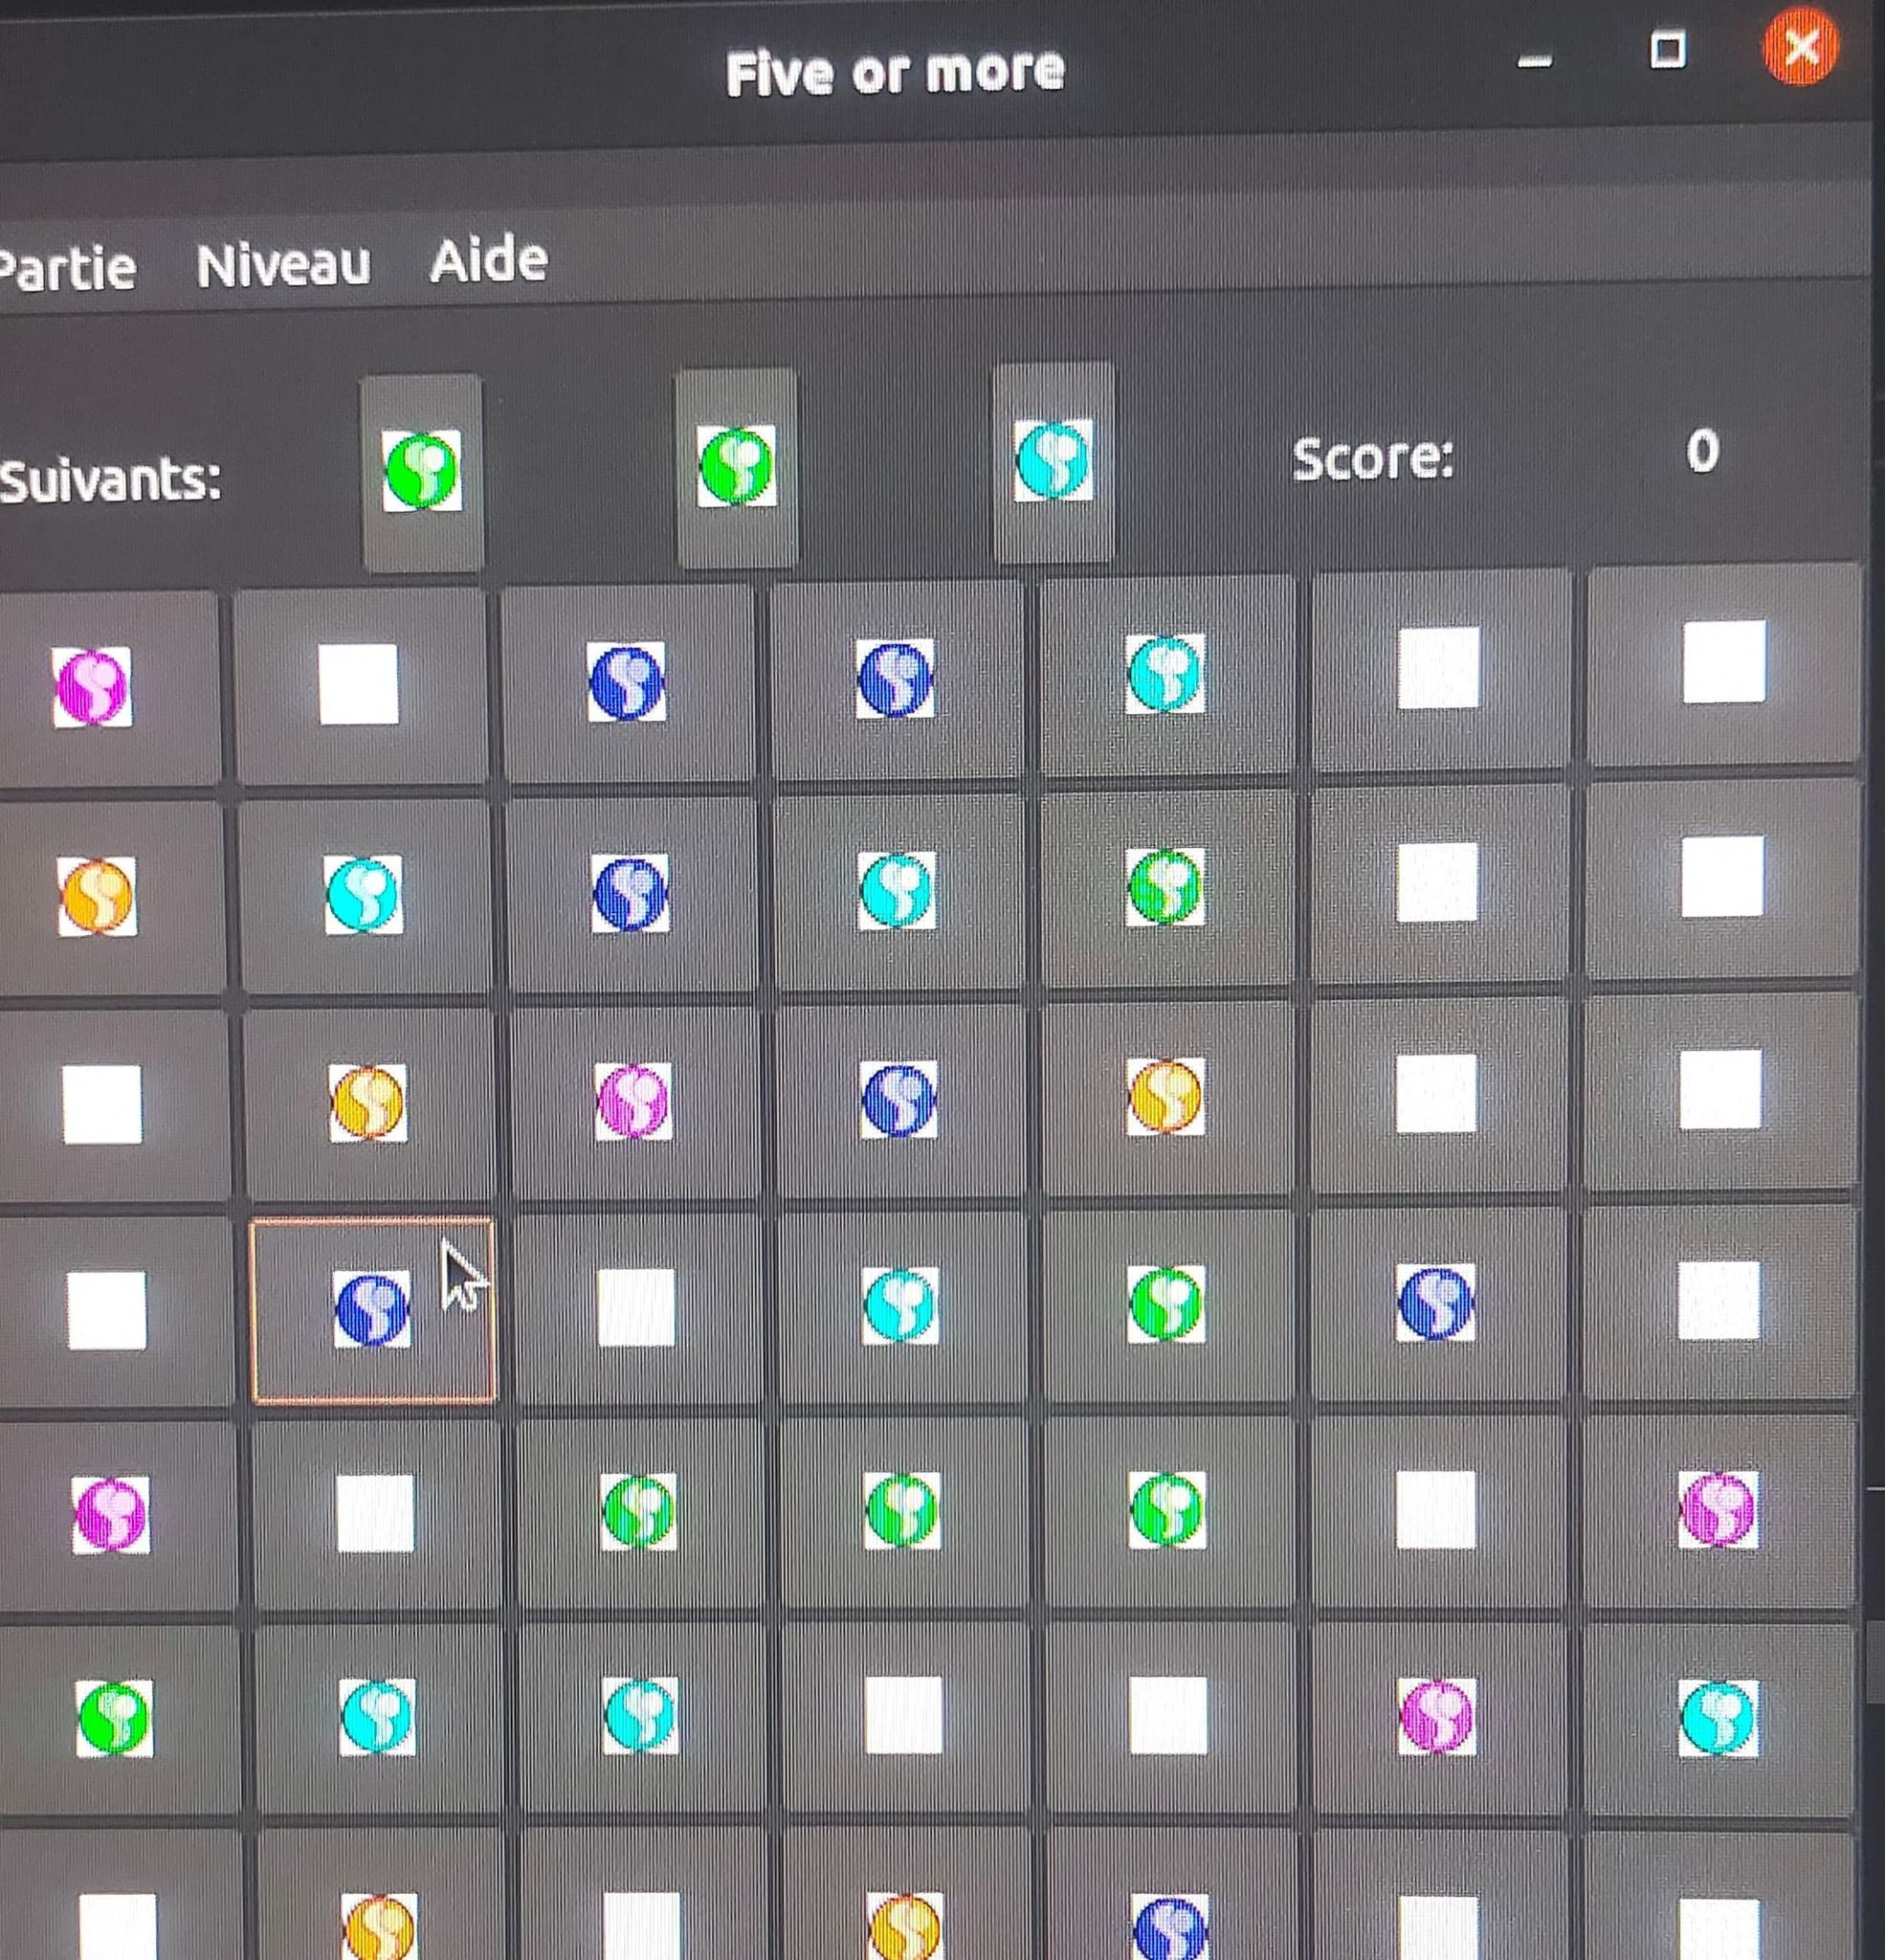
\includegraphics[width=4cm]{./images/facile.jpg}
    \end{subfigure}
    \begin{subfigure}[]{}
        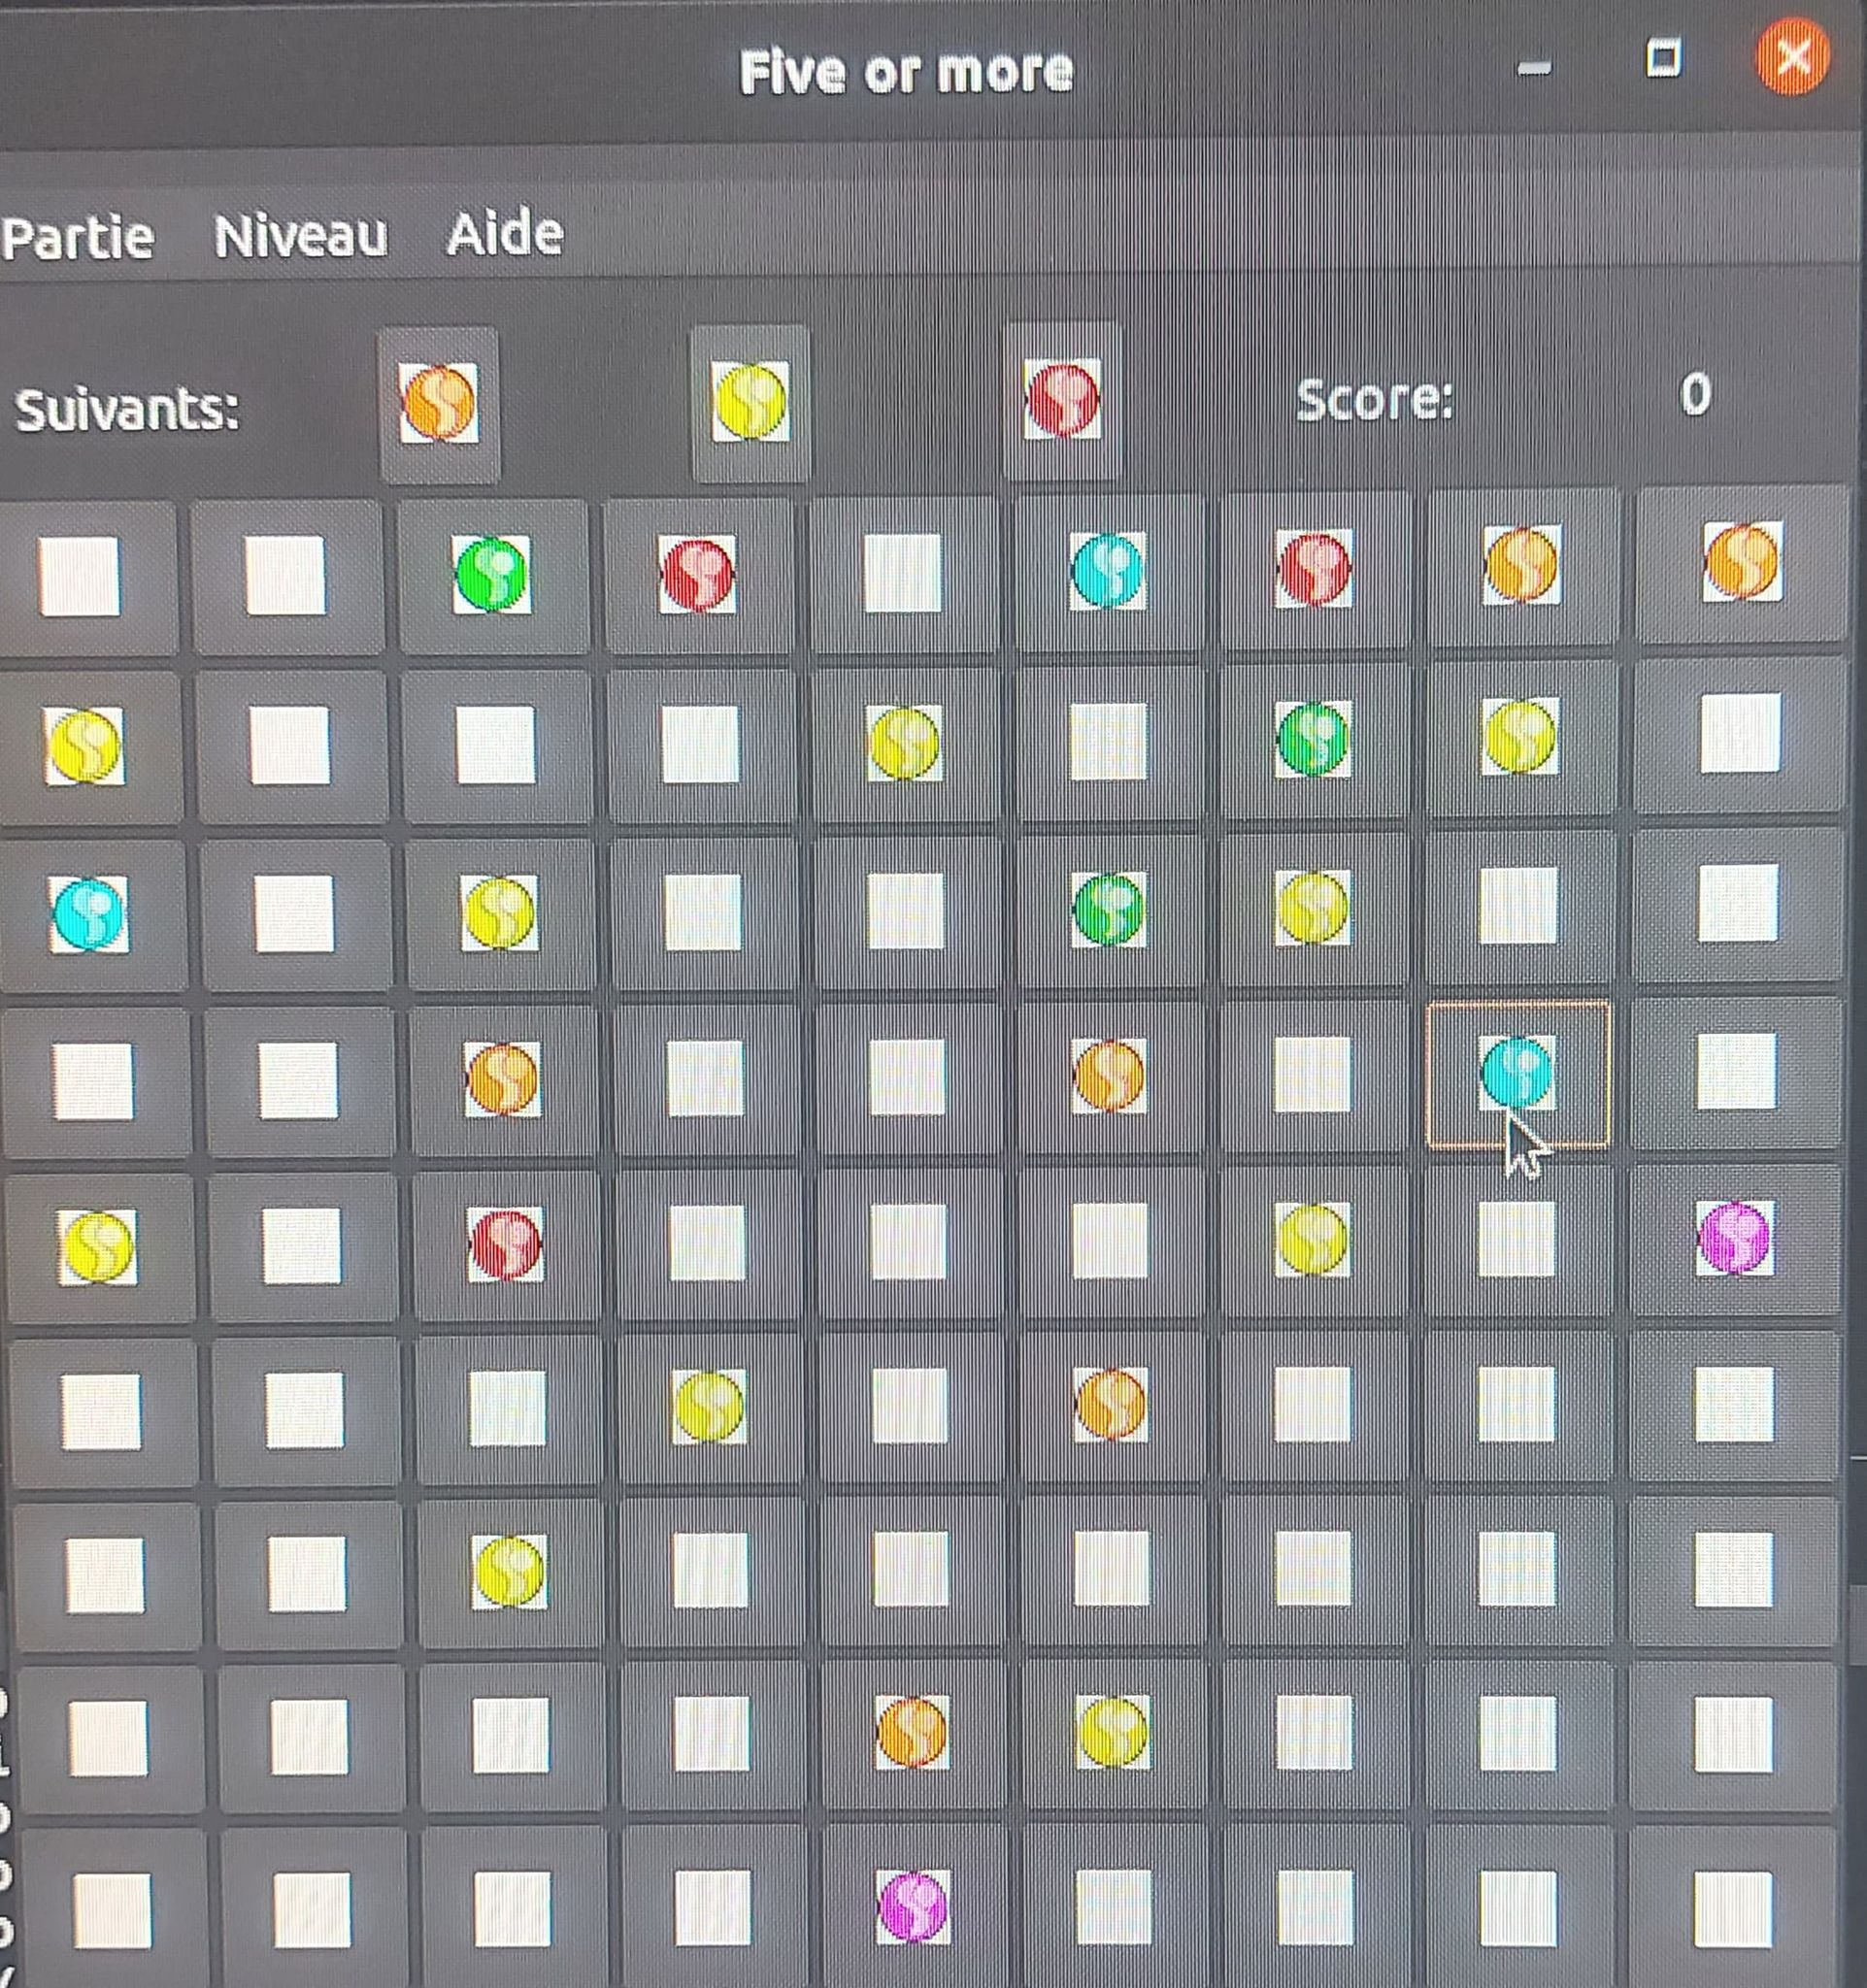
\includegraphics[width=4cm]{./images/moyen.jpg}
    \end{subfigure}
    \begin{subfigure}[]{}
        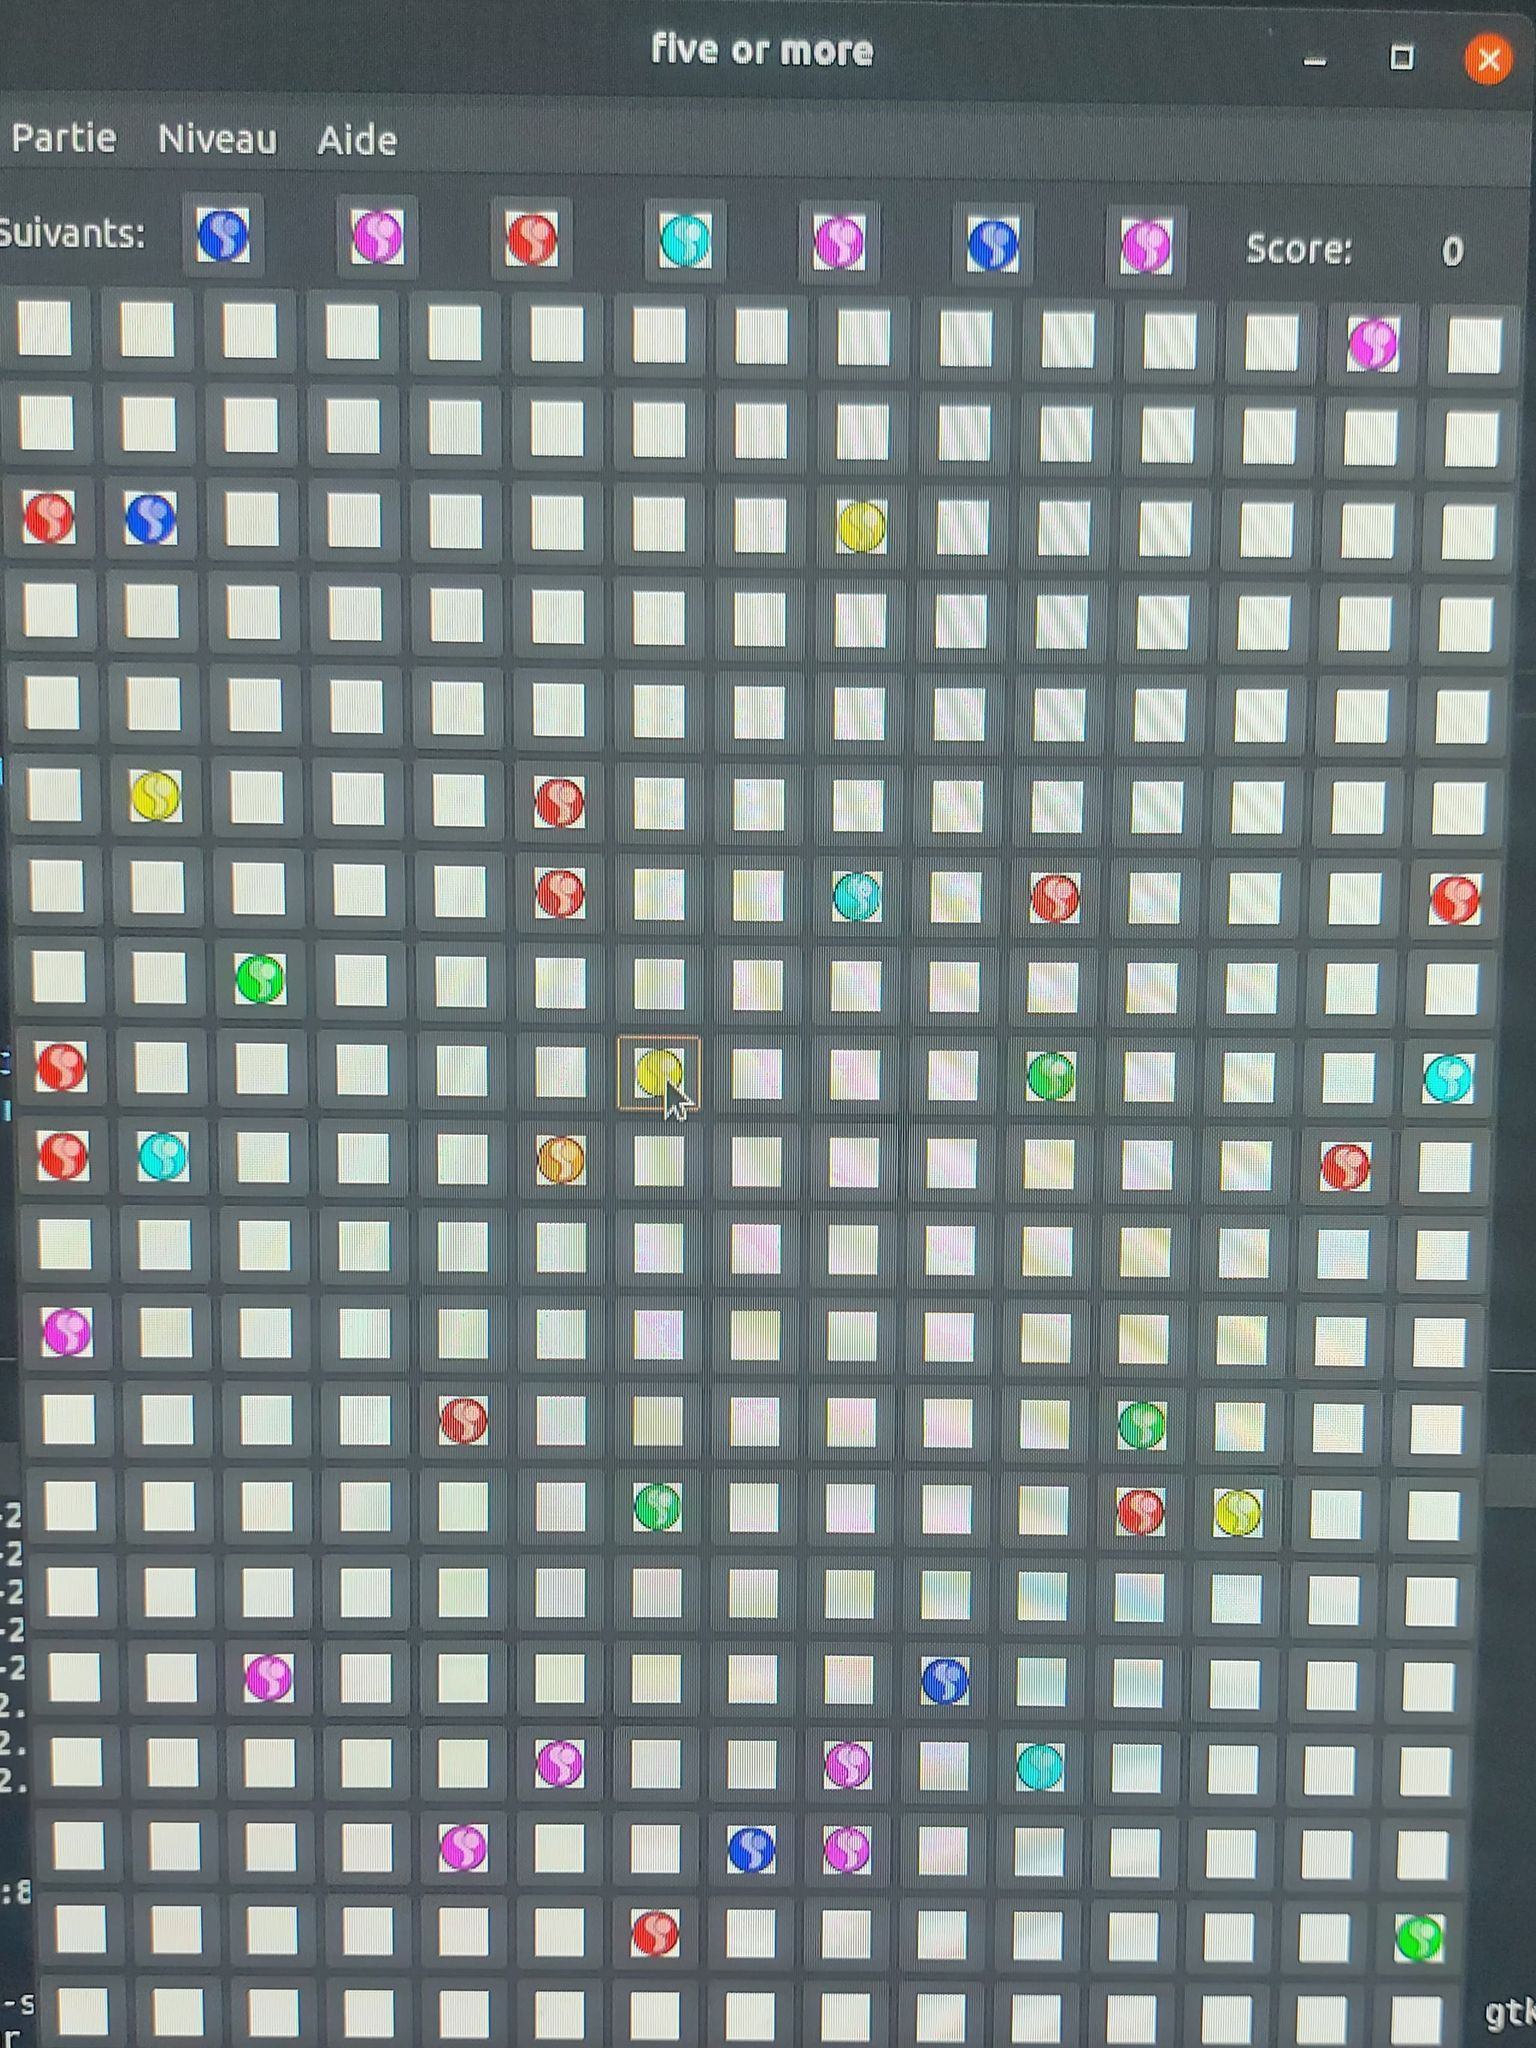
\includegraphics[width=4cm]{./images/difficile.jpg}
    \end{subfigure}

\end{figure}


\newpage

\subsection{Organisation du jeu}
\begin{figure}[!h]
    \centering
    \begin{subfigure}[]{}
        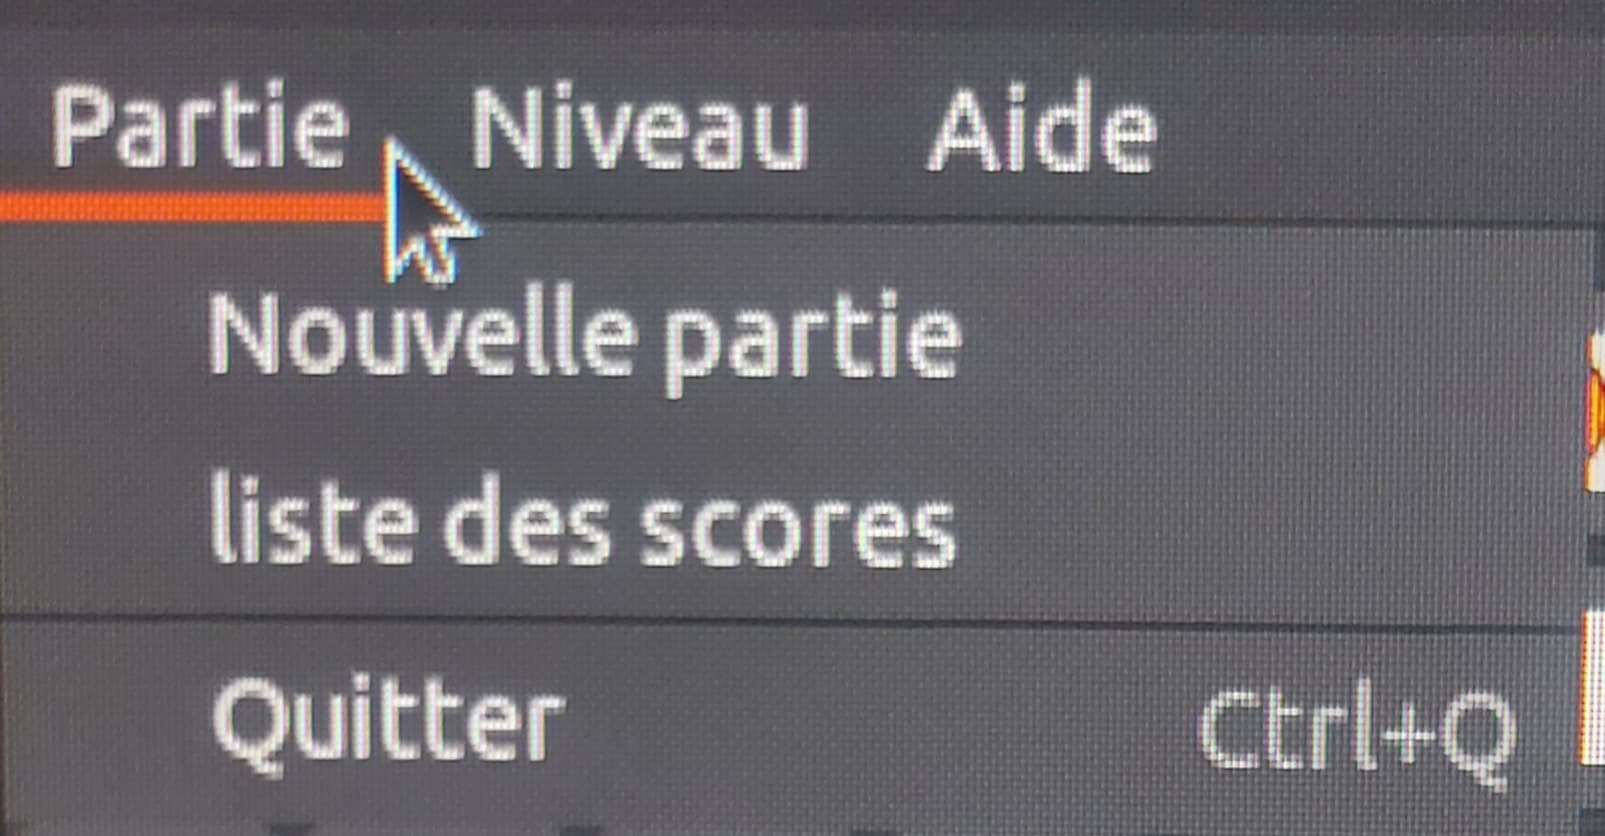
\includegraphics[width=4cm]{./images/partie.jpg}
    \end{subfigure}
    \begin{subfigure}[]{}
        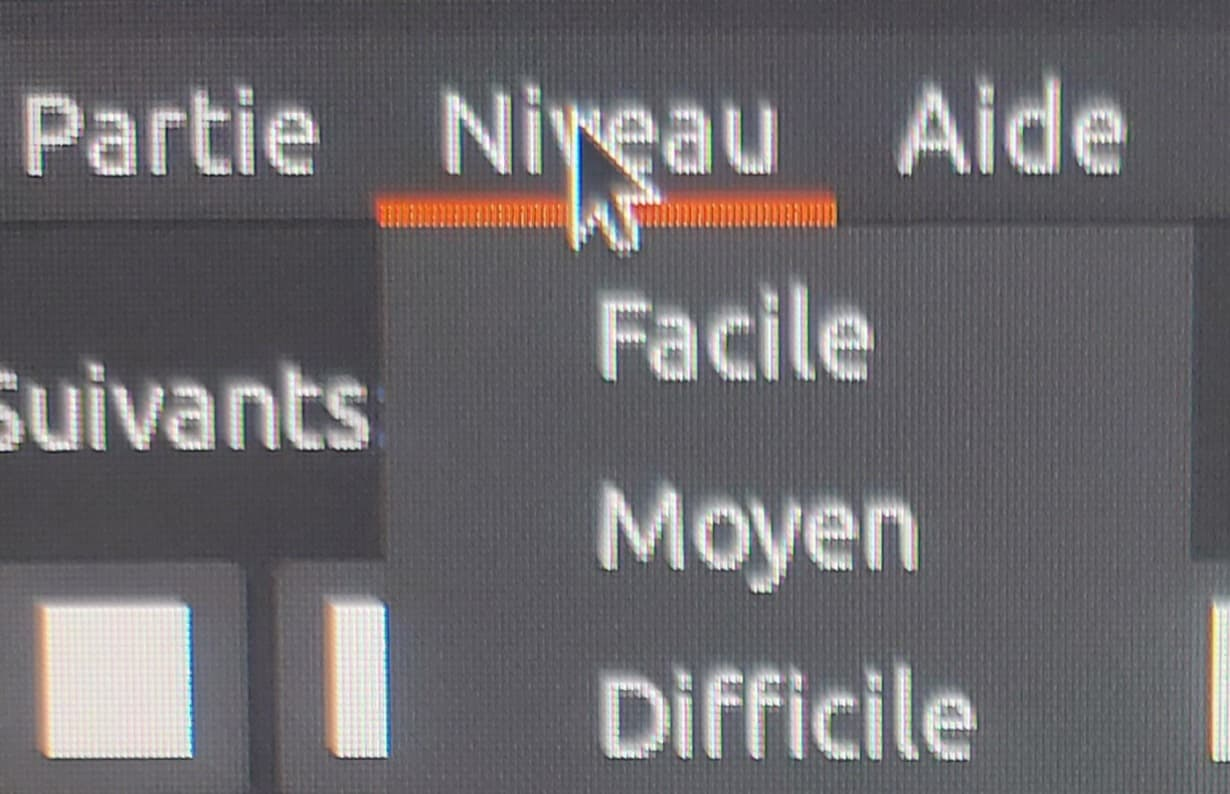
\includegraphics[width=4cm]{./images/niveau.jpg}
    \end{subfigure}
    \begin{subfigure}[]{}
        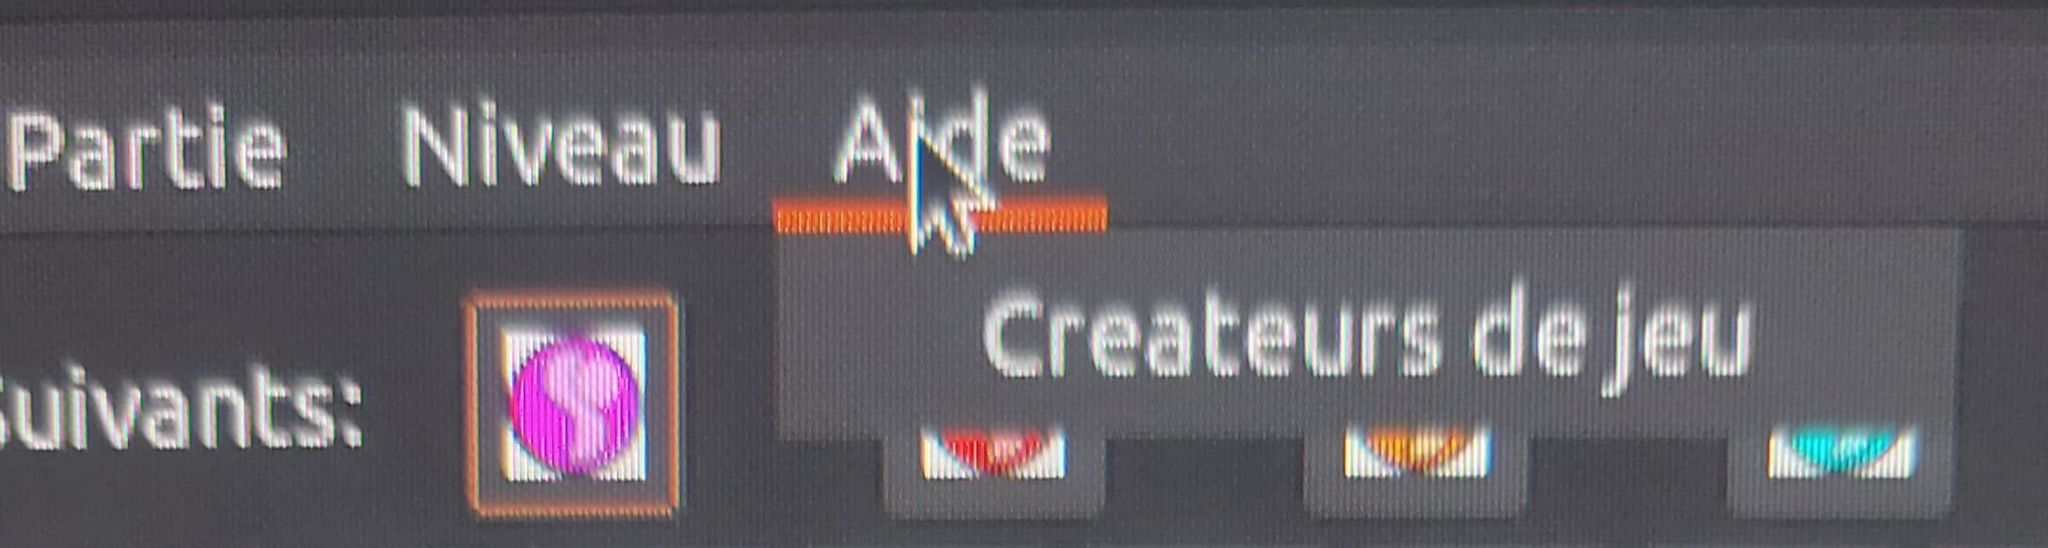
\includegraphics[width=4cm]{./images/createur1.jpg}
    \end{subfigure}

\end{figure}

\begin{figure}[!h]
    \centering
    \begin{subfigure}[]{}
        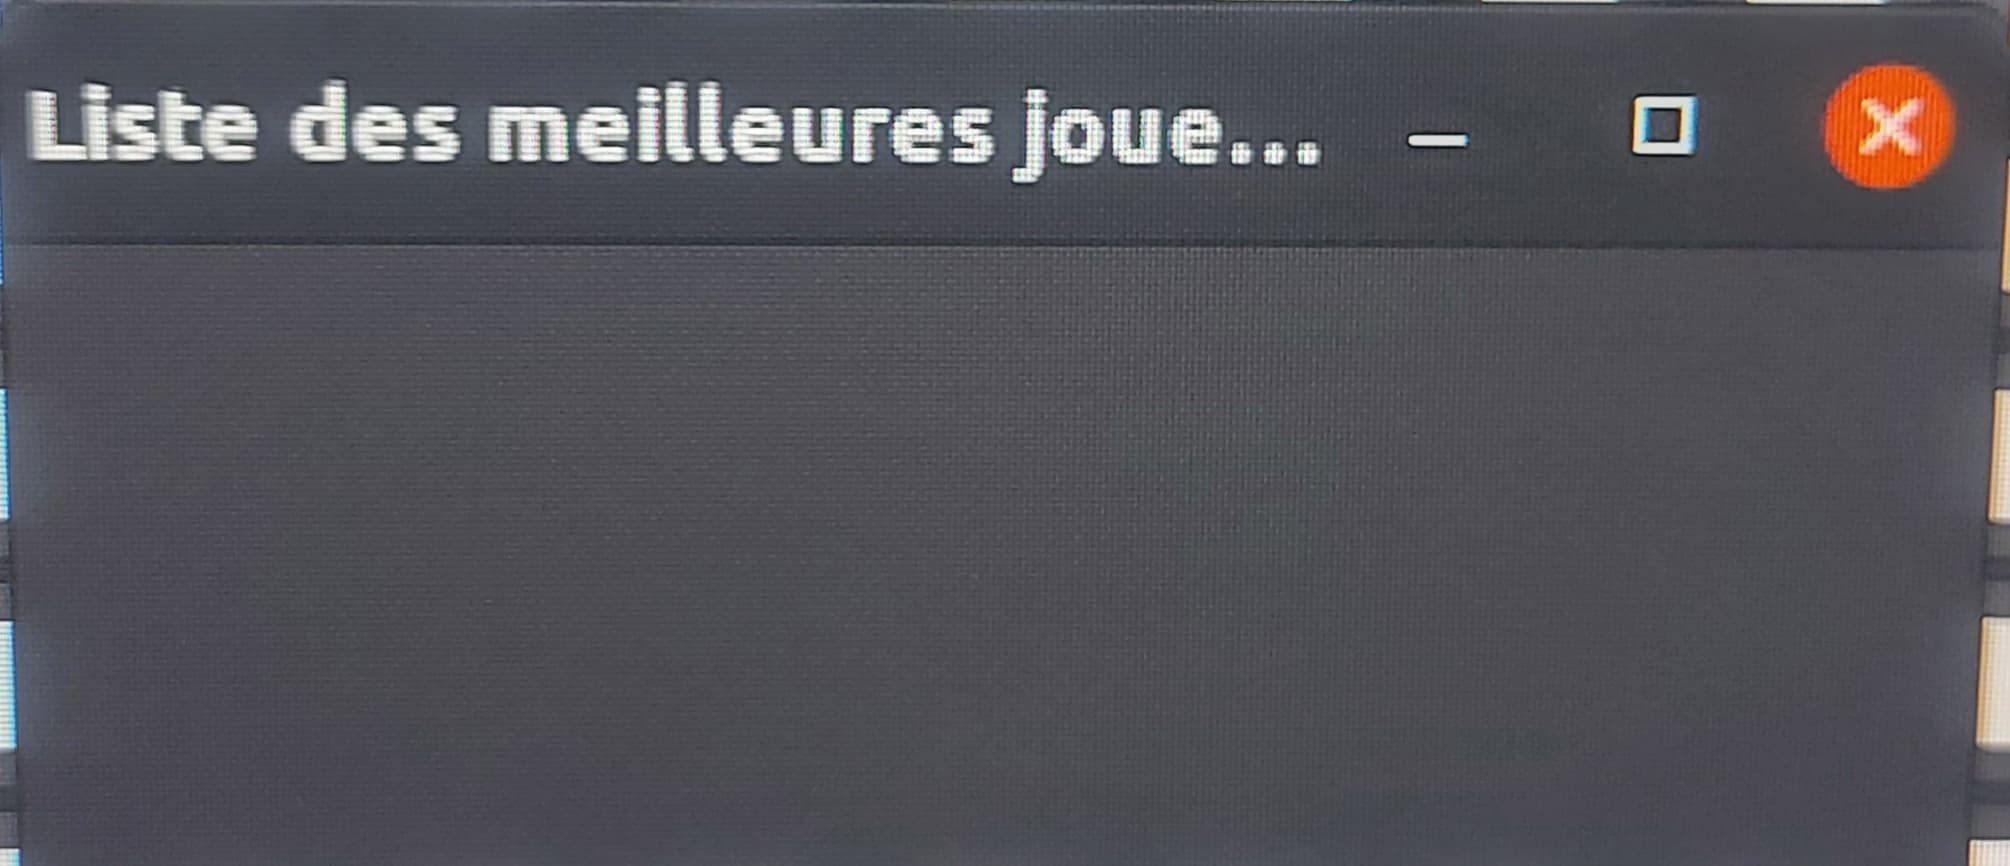
\includegraphics[width=4cm]{./images/liste_score.jpg}
    \end{subfigure}
    \begin{subfigure}[]{}
        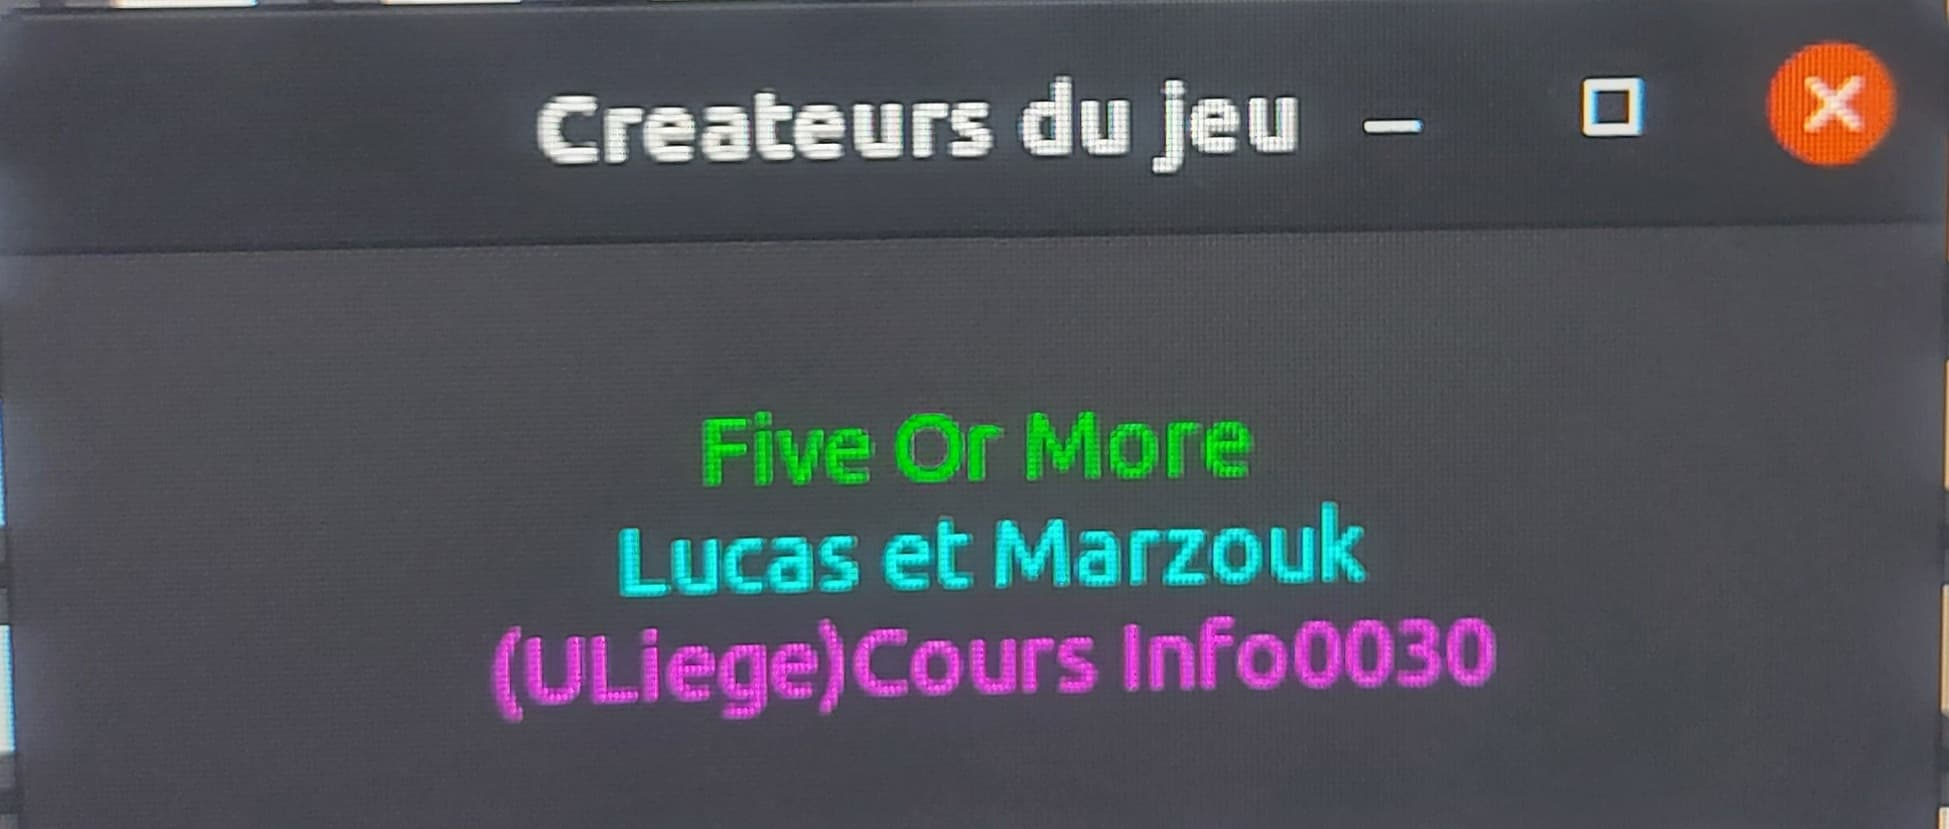
\includegraphics[width=4cm]{./images/createur2.jpg}
    \end{subfigure}
\end{figure}
La barre de menu contient 3 partie:
\newline
$\bullet$ L'image (h) : Nouvelle partie || liste des scores || Quitter
\newline
$\bullet$ L'image (i) : Facile || Moyen || Difficile
\newline
$\bullet$ L'image (j) : Createur du jeu 
\newline
$\bullet$ L'image (k) : Suite au click liste des scores, une fenêtre apparait et vous pouvez consulter les 10 meilleurs scores
\newline
$\bullet$ L'image (l) : Suite au click Createur du jeu, une fenêtre apparait et vous pouvez consulter des informations à propos des créateurs de ce fameux jeu.

\section{La gestion du code}
Pour le SCM gitlab, Lucas a créé le projet et a invité Marzouk à le rejoindre. Les débuts ont été compliqués au niveau de sa prise en main. Néanmoins, avec de la patience, nous avons su créé plusieurs branches pour chacun des patterns(Modele, Vue et Controleur) qui n'était pas la meilleure des solutions...Marzouk a incorporé tous les fichiers nécessaire pour travailler tranquillement dans chaucune des branches.Quand, nous avions fini
nous faisions 'git push' pour insérer les mises à jours que nous venions de faire.

\section{La coopération au sein du groupe}
Pour commencer, Lucas a commencé par coder l'interface graphique pour avoir un premier aperçu sur ce projet. Quand cele a été terminé, nous nous sommes partagés les taches pour savoir qui faisait quoi.De plus, pour plus de régularité, nous nous sommes données des deadlines afin de ne pas être débordé par les évènements.
Globalement, le projet s'est passé dans la bonne entente.

\section{Les améliorations possibles}
Nous avons eu des problèmes au niveau de la gestion du temps et nous avons du faire des sacrifices pour avoir un code qui 'fonctionne'. Le plus gros des problèmes se situe au niveau de la complexité de la victoire qui aurait pu être bien meilleure. Pour en rajouter, l'algorithme de déplacement se trouve incapable de réaliser certains déplacement complexe. Une amélioration pourrait être faite au niveau du premier click de l'utilisateur.Effectivement, il n'a pas le droit de changer d'avis sauf s'il fait délibérément un déplacement impossible.
Et enfin, la table de score n'est pas triée par soucis de temps ainsi que l'ajout des images aléatoire s'effectuent quand le score est incrémenté.

\section{Les éléments que nous avons appris}
Nous avons appris à utiliser git pour faciliter le travaille à plusieurs et sauvegarder nos données pour que l'autre membre du groupe puisse y accéder quand il le désire.En effet, se partager des fichiers sur discord n'est pas la meilleure des manières.\\
Le pattern MVC est une très bonne pratique a utilisé car sans lui nous aurions fait ce projet dans un seul et unique fichier ce qui serait ingérable.
Gtk, une bonne interface graphique, mais pas intuitive. De même, la prise en main a été faite par la recherche sur des forums, slides du prof ainsi que par des tiers. Grace à cette interface, nous avons pu créer ce jeu qui reste tout de même assez agréable à regarder et à jouer.
.Personnelement, j'ai appris que développer un jeu est loin d'être aussi facile que je le pensais et qu'il est important d'y réflechir avant de s'y attaquer la tête baissée.
\subsection{Conclusion}
Pour en finir, la réalisation du projet dans son ensemble a été agréable même s'il y avait quelque soucis au niveau de la gestion du temps.
\end{document}